\documentclass[12pt,openany,a4paper, titlepage]{article}

%import package
\usepackage[utf8]{inputenc}
\usepackage[T1]{fontenc}
\usepackage{lmodern}
\usepackage[french]{babel}
\usepackage{amsfonts,amsmath,amssymb,amsthm}
\usepackage{geometry} %fix the margin of the document
\geometry{top=3cm, bottom=3cm, left=2.5cm, right=2.5cm}
\usepackage{xargs}    %define new command
\usepackage{graphicx} %insertion image
\usepackage{caption}  %insertion de légendes et titres
\usepackage{indentfirst}
\usepackage{color}
\usepackage[table]{xcolor}
\usepackage{float}
\usepackage{tcolorbox}
\usepackage{appendix} % Appendices
\usepackage{tikz}

% Bibliographie
\usepackage[backend=biber,sorting=nyt,citestyle=numeric,bibstyle=alphabetic]{biblatex}% Bibliographie
\addbibresource{biblio.bib} 
\usepackage{csquotes}
\usepackage{url}

%title shape %\MakeUppercase
\usepackage{titlesec}
\titleformat{\chapter}[display]
{\normalfont\huge\bfseries\center}{\chaptertitlename\ \thechapter}{20pt}{\Huge}
\titleformat{\section}
{\normalfont\Large\bfseries\center}{\thesection}{1em}{}
\titleformat{\subsection}
{\normalfont\large\center}{\thesubsection}{1em}{}
\titleformat{\subsubsection}
{\normalfont\normalsize\bfseries\center}{\thesubsubsection}{1em}{}
\titleformat{\paragraph}[runin]
{\normalfont\normalsize\bfseries}{\theparagraph}{1em}{}
\titleformat{\subparagraph}[runin]
{\normalfont\normalsize\bfseries}{\thesubparagraph}{1em}{}

%news commands
\newcommand{\f}[2]{\frac{#1}{#2}}
\newcommand{\lp}{\left(}
\newcommand{\rp}{\right)}
\newcommand{\lb}{\left|}
\newcommand{\rb}{\right|}
\newcommand{\lc}{\left[}
\newcommand{\rcc}{\right]}
\newcommand{\la}{\left\langle}
\newcommand{\ra}{\right\rangle}
\newcommand{\dd}{\;\mathrm{d}}
\newcommand{\ddt}[1]{\frac{\partial #1}{\partial t}}
\newcommand{\R}{\mathbb{R}}
\newcommand{\C}{\mathbb{C}}
\newcommand{\Z}{\mathbb{Z}}
\newcommand{\N}{\mathbb{N}}
\newcommand{\HH}{\mathcal{H}}
\newcommand{\KK}{\mathcal{K}}
\newcommand{\spec}{\operatorname{spec}}
\newcommand{\res}{\operatorname{res}}
\newcommand{\specp}{\operatorname{spec_p}}
\newcommand{\essran}[1]{\operatorname{ess_{#1}ran}}
\newcommand{\esssup}[1]{\operatorname{ess_{#1}sup}}
\newcommand{\rd}{\mathbb{R}^d}
\newcommand{\vp}{\varphi}
\newcommand{\He}{H(\epsilon)}
\newcommand{\inv}{^{-1}}
\newcommand{\St}[2]{e^{-i #1 #2}}
\newcommand{\Stt}[2]{e^{i #1 #2}}
\newcommand{\ortho}{P^\perp}
\newcommand{\Ker}{\operatorname{Ker}}
\newcommand{\im}{\operatorname{Im}}
\newcommand{\pvm}{\mathrm{d}\langle \rangle}
\newcommand{\suminf}[2]{\sum_{#1=#2}^{+\infty}}
\newcommand{\limeo}{\lim\limits_{\epsilon \rightarrow 0^+}}

%new sections
\newtheorem{Def}{Définition}
\newtheorem{defprop}{Définition/Proposition}
\newtheorem{prop}{Proposition}
\newtheorem{theo}{Théorème}
\newtheorem{lem}{Lemme}
\theoremstyle{definition}
\newtheorem{ass}{Hypothèses}
\newtheorem{cor}{Corollaire}
\theoremstyle{definition}
\newtheorem{Not}{Notation}
\theoremstyle{definition}
\newtheorem{ex}{Exemple}
\theoremstyle{definition}
\newtheorem{exs}{Exemples}
\theoremstyle{definition}
\newtheorem{rem}{Remarque}
\newtheorem{postulat}{Postulat}
\theoremstyle{definition}

\newcommand{\HRule}{\rule{\linewidth}{0.5mm}} % Commande pour lignes horizontales

\everymath{\displaystyle}





\begin{document}

\begin{titlepage}
\begin{sffamily}
\begin{center}

% Upper part of the page. The '~' is needed because \\
% only works if a paragraph has started.

\includegraphics[scale=0.13]{logoCS.png}~\\[1.5cm]

\textsc{\LARGE Rapport de projet 3A}\\[1.5cm]

% Title
\HRule{} \\[0.4cm]
{\huge \bfseries La règle d'or de Fermi}
\HRule{} \\[1cm]

{\large Théo Duez}\\[2cm]

\begin{figure}[h]
    \begin{minipage}[c]{.5\linewidth}
    \centering
       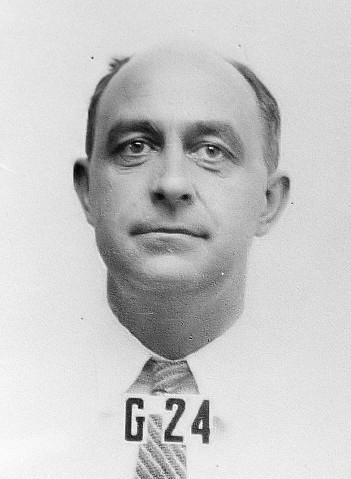
\includegraphics[height=7cm]{Enrico_Fermi.png} 
        \caption{Enrico Fermi}
    \end{minipage} \hfill
    \begin{minipage}[c]{.5\linewidth}
    \centering
        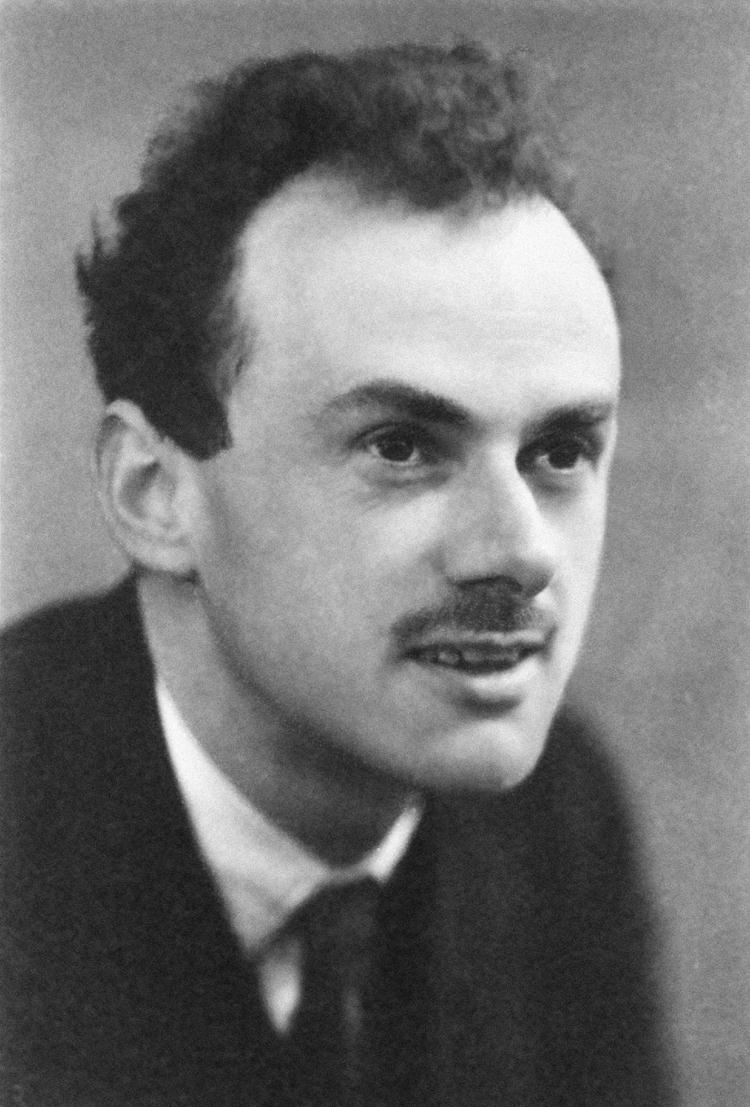
\includegraphics[height=7cm]{Paul_Dirac.jpg}
        \caption{Paul Dirac}
    \end{minipage}
\end{figure}\\[2cm]

% Author and supervisor
\begin{minipage}{0.4\textwidth}
\begin{flushleft} \large
Année scolaire 2023-2024
\end{flushleft}
\end{minipage}
\begin{minipage}{0.4\textwidth}
\begin{flushright} \large
\emph{Encadrant :} Antoine Levitt
\end{flushright}
\end{minipage}

\vfill

% Bottom of the page


\end{center}
\end{sffamily}
\end{titlepage}

\newpage

\section{Résumé}

Dans ce document, on s'intéresse à différentes preuves d'une règle de la physique quantique : la règle d'or de Fermi. Elle stipule qu'en présence d'une petite perturbation, à quelques conditions près, un état quantique quitte son état d'origine de façon irréversible avec une décroissance exponentielle en temps. Cette loi est bien connu du monde de la physique, mais des preuves rigoureuses et générales de cette loi sont à chercher du côté des mathématiciens. Différentes preuves existent et nous nous intéressons dans ce document à deux schémas de preuves complètement différents. La première utilise la théorie spectrale (approche par les résonances), la deuxième la théorie des équations aux dérivées ordinaires (approche de Davies). Cette règle d'or de Fermi ne peut exister que pour des systèmes de dimension infinie, mais devant faire des simulations sur ordinateur, je me suis posé quelques questions concernant le passage d'un système de dimension fini vers un système de dimension infini pour lequel la règle d'or de Fermi existe. L'exemple qui m'a intéressé en particulier est le modèle d'une chaîne 1D que l'on connecte par un site à un site extérieur.

\newpage

\tableofcontents

\newpage

\section{Introduction}

\subsection{Modélisation mathématique de la mécanique quantique}

Développé dans les années par une dizaine de physiciens devenus célèbres dont notamment Paul Dirac, Werner Heisenberg, Louis de Broglie, Erwin Schrödinger etc.,  la mécanique quantique est la branche de la physique théorique qui permet d'expliquer le comportement des particules élémentaires, des atomes, des molécules ou de tout système physique de taille similaire. Elle a rencontré de nombreux succès en permettant d'expliquer ce que la physique classique ne pouvait pas, par exemple la structure électronique des atomes et des molécules, .... . 

Nous ne prétendons pas ici à fournir ne serait-ce qu'une introduction d'introduction d'un vrai cours de mécanique quantique, et bon nombre de concepts et de résultats élémentaires seront omis. Pour plus de détails, nous renvoyons le lecteur à \cite{Quantum} et\cite{Levitt}. Nous allons juste nous concentrer sur ce que l'on appelle les postulats de la mécanique quantique qui permettent de poser les bases de la modélisation mathématique et de ses outils avec lesquels nous allons traiter tout au long de ce rapport.

\vspace{3mm}
\begin{tcolorbox}[colback=gray!5!white,
                  colframe=gray!80!white,
                  title= Postulat 1 : Principe de superposition ]
L'état d'un système quantique est défini à tout instant $t$ par un vecteur unitaire, dénoté $|\psi(t)\rangle$, appartenant à un espace de Hilbert complexe $\HH$ séparable. Deux états qui différent d'un facteur de phase $e^{i\theta}$ pour $\theta\in[0,2\pi)$ représentent le même état.
\end{tcolorbox}
\vspace{3mm}

\begin{rem}
    Il est usuel en mécanique quantique de noter un vecteur 
    de $\HH$ aussi bien $\psi$ que $|\psi\rangle$. Il s'agit d'un "ket". En notant la forme linéaire associé à ce vecteur par $\langle\psi |$, i.e l'application $u\in\HH \mapsto \langle \psi | u\rangle$ appelé un "bra", on obtient que les notations coïncident avec le produit scalaire et sont très utiles en pratique. Par exemple, le projecteur sur la droite vectoriel engendrée par $|\psi\rangle$ est $|\psi\rangle\langle\psi |$.
\end{rem}

\begin{exs}
    Donnons quelques exemples d'espaces d'états.
    \begin{enumerate}
        \item[1] $\C$ est l'espace de Hilbert séparable le plus simple que l'on puisse considérer. Comme deux complexes de module 1 différent toujours d'un facteur de phase, cet espace est trivial puisque constituer que d'un seul état.
        \item[2] $\C^2$ est quant à lui l'espace non trivial le plus simple que l'on puisse considérer. Soit $|\psi\rangle = (re^{i\vp}, r'e^{i\vp'}) \in \C^2$ avec $r,r'\geq 0$ et $\vp, \vp' \in [0,2\pi)$. Quitte à multiplier par le facteur de phase $e^{-i\vp}$ (qui ne change pas l'état du système, on peut supposer $\vp = 0$. Comme un vecteur d'état est de norme 1, on a que $r^2 + r'^2 = 1$ et il existe donc $\theta \in [0,2\pi[$, que l'on peut réduire à $\theta \in [0,\pi[$ une nouvelle fois par invariance par multiplication par un facteur de phase, tel que $|\psi\rangle = \lp \cos(\theta), \sin(\theta)e^{i\vp'}\rp$. Une telle paramétrisation fait que l'on appelle cet espace d'état la sphère de Bloch, qui permet de modéliser par exemple les qubits, composants de base en théorie de l'information quantique.
        \item[3] De même, on peut considérer $\C^n$ pour $n\in\N$. Un tel espace peut modéliser un système qui peut se déplacer/propager sur un ensemble de $n$ sites.
        \item[4]  De façon plus général, si l'on souhaite considérer un système qui évolue sur une chaîne discrète infinie, l'espace approprié à considérer est $\ell^2(\Z)$, l'espace des suites sur $\Z$ de carré intégrable, qui est bien, muni sa norme euclidienne, un espace de Hilbert séparable. On peut aussi considérer $\ell^2(A)$ où $A$ est un ensemble dénombrable.
        \item[5] Un dernier exemple est l'espace $L^2(\R^d,\C)$ où $d\in\N$, l'espace des fonctions de $R^d$ vers $\C$ de carré intégrable. Cet espace est un espace de Hilbert séparable pour sa norme euclidienne. C'est l'espace typique utiliser si l'on souhaite par exemple modéliser un système dont la position varie dans un continuum, ici $\R^d$.
    \end{enumerate}
\end{exs}

\begin{rem}
    Expliquons pourquoi on demande à ce que $|\psi(t)\rangle$ soit de norme constante égale à $1$ au cours du temps. Cela est due au fait bien connue que la mécanique quantique est une description probabiliste de la physique. Si par exemple $\HH = \ell^2(A)$, on doit donc avoir $||\psi(t)||^2 = \sum_{a\in A} |\psi_a(t)|^2$ et si ou bien $\HH = L^2(\R^d,\C)$, on doit avoir $\int_{\R^d}|\psi(t,x)|^2dx = 1$. Dans le premier cas, on doit penser $|\psi_a(t)|^2$ une probabilité sur l'atome (au sens mathématique) $\{a\}$ et $|\psi(t,x)|^2$ plutôt la une densité de probabilité au point $x \in \R^d$. La position moyenne d'une particule se mouvant dans $A$ s'écrit donc par théorème de transfert $\sum_{a\in A} a|\psi_a(t)|^2$ et si elle se meut dans $\R^d$ elle s'écrit $\int_{\R^d}x|\psi(t,x)|^2dx$.
\end{rem}

\vspace{3mm}
\begin{tcolorbox}[colback=gray!5!white,
                  colframe=gray!80!white,
                  title= Postulat 2 : Principe de correspondance ]
A tout observable classique correspond un opérateur linéaire $A$ autoadjoint sur $\HH$.
\end{tcolorbox}
\vspace{3mm}

\begin{rem}
    $A$ est simplement une matrice si $\HH$ est de dimension finie mais peut être un opérateur possiblement non borné si $\HH$ est de dimension infinie. L'étude de tels opérateurs, et à l'instar des matrices de leur spectre et diagonalisabilité, fait l'objet de la théorie dite spectrale dont nous ferons un très rapide tour dans la section suivante. Ici autoadjoint est une généralisation à la dimension infinie de la notion d'hermitianité pour les matrices complexes.
\end{rem}

\begin{ex} 
Donnons quelques exemples pour des systèmes vivant dans l'espace le plus intéressant, $L^2(\R^d,\C)$ où $d\in\N$. A titre d'exemple, considérons que le système est constitué d'un électron libre.
\begin{enumerate}
    \item[1] Parler de la position, au sens classique, de l'électron en mécanique quantique n'a pas de sens puisque l'état d'un système est représenté uniquement par un vecteur $|\psi\rangle$ de l'espace de Hilbert $\HH$, ici une fonction définie sur tout $\R^d$. C'est d'ailleurs pourquoi on entend parler en mécanique quantique du "nuage électronique". En mécanique quantique, la position est un opérateur $X$ définie comme $$X|\psi\rangle = x\in \R^d \mapsto x|\psi\rangle(x) \in \C$$ de sorte qu'avec la remarque précédente, la position moyenne s'écrit $$ \langle \psi | X | \psi \rangle.$$ En fait, on appelle moyenne de l'observable $A$, la quantité $\langle \psi | A | \psi \rangle$, ce qui justifie la définition de l'opérateur position. On remarque que l'opérateur $X$ est bien un opérateur autoadjoint : soit $\psi_1, \psi_2 \in \HH$
    \begin{equation}
        \la\psi_1, X\psi_2\ra =\int_{\R^d}\overline{\psi_1(x)}x\psi_2(x) \dd x
        = \int_{\R^d}\overline{x\psi_1(x)}\psi_2(x) \dd x 
        = \la X\psi_1, \psi_2\ra.
    \end{equation}
    \item[2] De même, parler du moment (masse $\times$ vitesse) de l'électron n'a pas de sens. Quelle définition peut-on donner à l'opérateur $P$ correspondant ? L'idée naturelle est de poser que les quantités moyennes "vérifient" les principes classiques, ici que la dérivée de la position est égale au moment (en se plaçant dans un système d'unité où la masse $m$ de l'électron est telle que $m=1$ :
    $$ \langle \psi |P|\psi\rangle = m\frac{\dd \langle \psi | X | \psi\rangle}{\dd t}.$$
    Nous verrons après le sixième postulat un théorème permettant de calculer explicitement le terme de droite.
\end{enumerate}
\end{ex}


\vspace{3mm}
\begin{tcolorbox}[colback=gray!5!white,
                  colframe=gray!80!white,
                  title= Postulat 3 : Principe de quantification ]
Quelque soit l'état du système, la mesure d'une observable $A$ ne peut être qu'une valeur propre de l'observable $A$.
\end{tcolorbox}
\vspace{3mm}

\begin{rem}
    Lorsque l'on parle ici de mesure, il s'agit bien là d'une mesure physique réalisé à l'aide d'instruments et sous intervention humaine, ce qui est un point déroutant en mécanique quantique. 
\end{rem}

\begin{rem}
    Une remarque importante doit être faite concernant le spectre des opérateurs. S'il est aisé d'étudier le spectre des matrices, étudier le spectre d'opérateur de dimension infinie et possiblement non borné est beaucoup plus délicat et se traite dans des cours de théorie spectrale. Un exemple d'un tel cours est \cite{Macher}. Donnons ici quelques aperçus. Ce qui fait que l'analyse spectrale en dimension infinie est beaucoup plus délicate est due au fait de la présence de phénomènes complètement absents en dimension finie. Déjà, une première difficulté vient de la définition du spectre. Le spectre d'une matrice carré $M$ peut être définie comme l'ensemble des complexes tel que $M-z$ ne soit pas inversible. C'est aussi équivalent à demander que $M-z$ ne soit pas subjective, ou encore non injective. En dimension infinie, aucune des ces définitions n'est équivalente. Le spectre est donc constitué de plusieurs parties, chacun correspondant à une facette du problème qui empêche $H-z$ d'être inversible (et d'inverse borné). Une partie de ce spectre, noté , $\sigma(H)$ ressemble à celui que l'on connaît en dimension finie : les valeurs propres de multiplicité finie, constituant le spectre dit discret et noté $\sigma_d(H)$. Mais il y a aussi les valeurs propres de multiplicité infinie qui corresponde au cas d'un point d'accumulation. On a aussi qu'une partie du spectre empêche $H-z$, comme opérateur de $\mathcal{H}$ dans $\mathcal{H}$, d'être surjective et dedans comprend un spectre continue, par exemple un intervalle de $\R$. Il est possible de décomposer le spectre en différents types et c'est ce qui est fait toute la richesse de l'analyse spectrale en dimension infinie.
\end{rem}

\begin{exs}
    Donnons plusieurs exemples.
    \begin{enumerate}
        \item[1] Une matrice possède un spectre constituée entièrement de valeurs propres de multiplicités finies.
        \item[2] L'opérateur position, lui, ne possède pas de valeur propre. En effet, si c'était le cas, on aurait qu'il existe $\lambda\in\C$ et $\psi\in L^2(\R,\C)$ non nul  tels que $X|\psi\rangle = \lambda |\psi\rangle$. En évaluant en $x\in\R$, on a alors $\lambda |\psi\rangle(x) = x|\psi\rangle(x)$ et comme $\psi$ est non nul, il existe un $x$ tel que $\psi\rangle(x)$ soit non nul et on trouve alors que $\lambda = x$. Ce qui signifierait que $\psi$ est non nul qu'en un seul point $x\in\R$, c'est à dire que c'est la fonction nulle dans $L^2(\R,\C)$, ce qui n'est pas possible. Cependant, l'opérateur position possède toute fois un spectre. Intuitivement, chaque point $x\in\R$ semble jouer presque un rôle de valeur propre. Ici, $\R$ constitue le spectre continue de l'opérateur $X$.
    \end{enumerate}
\end{exs}

\vspace{3mm}
\begin{tcolorbox}[colback=gray!5!white,
                  colframe=gray!80!white,
                  title= Postulat 4 : Principe de décomposition spectrale ]
La mesure d'une observable $A$ est une variable aléatoire dont la loi est donnée par $$\mathbb{P}(\text{mesurer} \in E) = ||P_A(E)\psi||^2$$
où $E$ est un borélien de $\HH$ (où la topologie est celle induite par la norme) et $P_A$ la mesure spectrale de l'opérateur $A$.  
\end{tcolorbox}
\vspace{3mm}

\begin{rem}
    La formulation rigoureuse donnée dans ce postulat diverge quelque peu de celles que l'on peut trouver généralement dans des livres de physiques qui se concentrent avec des formulations plus simples mais moins clair mathématiquement. Pour cause, la notion de mesure spectrale est une notion dont les résultats sous-jacent demandent pas mal de travail. Encore une fois, nous référons à la section suivante pour un rappel de théorie spectrale. Expliquons toutefois intuitivement ce qu'est la mesure spectrale d'un opérateur.
\end{rem}

\vspace{3mm}
\begin{tcolorbox}[colback=gray!5!white,
                  colframe=gray!80!white,
                  title= Postulat 5 : Principe de réduction du paquet d’onde ]
Immédiatement après une mesure de l'observable $A$, l'état du système est donnée par la formule $\f{P_A(E)\psi}{||P_A(E)\psi||}$.
\end{tcolorbox}
\vspace{3mm}

\begin{rem}
    Encore une fois, l'expérience de la mesure modifie le système quantique. Le postulat précédent dit que le système se retrouve projeté dans le sous-espace propre généralisé. 
\end{rem}

\vspace{3mm}
\begin{tcolorbox}[colback=gray!5!white,
                  colframe=gray!80!white,
                  title= Postulat 6 : Evolution d'un système dans le temps ]
Entre toute mesure, l'évolution de l'état d'un système quantique est régit par l'équation de Schrödinger 
$\partial_t \psi(t) = H(t)\psi(t)$
où $H(t)$ est l'opérateur correspondant à l'hamiltonien du système à l'instant $t$, i.e à l'observable "énergie total".
\end{tcolorbox}
\vspace{3mm}

\begin{rem}
    \begin{enumerate}
        \item[1] L'existence de solutions à un tel équation est donné par le théorème de Stone que nous verrons dans la section suivante sur les rappels de théorie spectrale.
        \item[2] Ce postulat permet de donner le théorème suivant :
        \begin{theo}[Théorème d'Ehrenfest]
        Si $A$ est un opérateur autoadjoint de $\HH$ indépendant du temps, alors pour tout $\psi\in\HH$
        \begin{equation}
            \frac{\dd \langle \psi | A | \psi\rangle}{\dd t} = \langle \psi | [A,H] | \psi\rangle
        \end{equation}
        où $[\cdot,\cdot]$ est le crochet de Lie usuel.
    \end{theo}
    Ainsi, on peut compléter la remarque précédente et donner l'expression de l'opérateur moment, sachant que l'opérateur $H$ pour l'espace $L^2(\R^d,\C)$ est supposé, comme toujours, contenir le terme d'énergie cinétique représenté par le laplacien $\Delta$:
    \begin{equation}
        P = -i\nabla
    \end{equation}
    qui se trouve via une intégration par partie.
    \end{enumerate}
\end{rem}


\subsection{Perturbations}

Nous présentons maintenant une autre notion beaucoup étudiée en mécanique quantique : les perturbations.
En effet, en physique quantique, il arrive souvent que le système que l'on étudie sois soumis à une perturbation. Par exemple, si une particule, initialement libre, se retrouve soumise à un potentiel. Lorsque l'on parle de perturbation, il est souvent entendu qu'elle est petite, il s'agit vraiment d'une perturbation et est souvent facteur d'un réel positif $\epsilon$ pour contrôler l'amplitude de la perturbation.
Concrètement, un perturbation signifie que notre hamiltonien de départ $H_0$ se retrouve remplacé par un nouvel hamiltonien $H(\epsilon) := H_0 + \epsilon H_1$ où $H_1$ est aussi un opérateur autoadjoint représentant la perturbation. Étant donné que les valeurs propres des opérateurs jouent un rôle centrale en mécanique, puisque pour rappel ceux sont les seules informations que l'on peut mesurer, il faut donc étudier les valeurs propres de l'hamiltonien perturbé. Plusieurs théories permettent de tels études selon les caractéristiques de la perturbation. On peut par exemple la théorie des perturbations classiques, souvent présenté en cours de physique, et les théories de Kato et de la diffusions, présentés dans des cours de théorie spectrale. Dans ce projet, nous serons amené à étudier l'évolution de valeurs propres avec la perturbation.

\newpage
\subsection{La règle d'or de Fermi} 

Maintenant que nous avons rappelé les principes de la modélisation mathématique de la mécanique quantique, nous pouvons présenter le sujet de ce projet : la règle d'or de Fermi. \\

Cette règle stipule que si un système, se trouvant dans un état propre énergétique, subit une perturbation, celui-ci peut, sous certaine hypothèses sur cette perturbation, soit rester dans l'état initiale avec une probabilité de 1 à un $o_\epsilon(1)$ près qui est uniforme en temps, soit quitter irréversiblement cet état initial vers un continuum d'états propres de façon exponentielle en temps à un $o_\epsilon(1)$ près qui est toujours uniforme en temps.\\


Rentrons maintenant dans le formalisme mathématique. Nous allons pour cela considérer un système initial régit par un hamiltonien $H_0$ sur un espace de Hilbert $\mathcal{H}$, dont le produit scalaire hermitien est noté $\langle \cdot, \cdot, \rangle$ et la norme $||\cdot ||$. L'état initial à $t=0$ est $\vp_0$ qui est un vecteur propre de $H_0$ pour la valeur propre $\lambda_0$. On note $\mathcal{K}_0$ le sous-espace propre associé et $m$ sa dimension. Dans la décomposition $\mathcal{K}_0 \oplus \mathcal{K}_0^\perp$, l'hamiltonien s'écrit :
\begin{equation}
    H_0 = \begin{pmatrix}
\lambda_0I_m & 0 \\
0    & A 
\end{pmatrix}
\end{equation}
où $A$ est un opérateur auto-adjoint de $\mathcal{K}_0^\perp$. Il est important de noter qu'ici $\lambda_0$ ne peut pas être une valeur propre de $A$ mais appartenir à son spectre. Ce système va subir dès l'instant $t=0$, une perturbation $\epsilon H_1$ d'amplitude $\epsilon$ qui s'écrit dans la décomposition $\mathcal{K}_0 \oplus \mathcal{K}_0^\perp$ :
\begin{equation}
    H_1 = \begin{pmatrix}
B        & \Gamma \\
\Gamma^* &  C
\end{pmatrix}
\end{equation}
où $B$ et $C$ sont des opérateurs auto-adjoints respectivement de $\mathcal{K}_0$ et $\mathcal{K}_0^\perp$, et où $\Gamma$ est une application linéaire borné de $\mathcal{K}_0^\perp$ vers $\mathcal{K}_0$, et $\Gamma^*$ sont application adjointe. L'évolution du système est donc régit par l'hamiltonien
\begin{equation}
    H(\epsilon) = H_0 + \epsilon H_1
\end{equation}
de sorte que, si $\vp(t)$ est l'état du système à l'instant $t$, on ait pour tout $t\geq 0$ :
\begin{eqnarray}
    \vp_\epsilon(t) = e^{-iH(\epsilon)t}\vp_0.
\end{eqnarray}

Dans notre projet, on s'intéresse à étudier la probabilité de trouver l'état du système à l'instant $t$ dans l'état initiale. Cette probabilité s'écrit, en vertu des postulats de la mécanique quantique :
\begin{equation}
    |\la \vp_0, \vp_\epsilon(t) \ra |^2.
\end{equation}

La règle d'or de Fermi a pour but de donner une approximation à l'ordre zéro en $\epsilon$  de cette dernière quantité, approximation qui est uniforme en temps. Elle dit que sous certaines hypothèses, on a

\begin{equation}
    |\la \vp_0, \vp_\epsilon(t) \ra |^2 = e^{2\Gamma(\epsilon)t} + o_\epsilon(1)
\end{equation}
où $\Gamma(\epsilon)$ est un coefficient réel négatif. 


\begin{ex}
Pour illustrer, nous allons nous appuyer sur un modèle en particulier : celui d'une chaîne 1D reliée faiblement à un site. Ce modèle est modélisé par l'espace de Hilbert $\C\oplus\ell^2(\Z,\C)$ et l'hamiltonien écrit sur cette décomposition:
\begin{equation}
    H_{chaine} = \underbrace{\begin{pmatrix}
E & 0 \\
0 & A 
\end{pmatrix}}_{H_0} \,+\, \epsilon
\underbrace{\begin{pmatrix}
0        & e_{R_0} \\
e_{R_0}^* &  0
\end{pmatrix}}_{H_1}
\end{equation}
où $E\in\R$, $R_0\in\Z$, $A$ est l'opérateur auto-adjoint de $\ell^2(\Z,\C)$ définit par 
\begin{equation}
    (Au)_n = u_{n+1} + u_{n-1}
\end{equation}
pour $n\in\Z$ et où $\lp e_i\rp_{i\in\Z}$ est la base canonique de $\ell^2(\Z,\R)$ et $\lp e_i\rp_{i\in\Z}^*$ sa base duale. En repérant par $(z,u)$ un élément de $\C\oplus\ell^2(\Z,\C)$, l'état initial est $(1,0)$ qui est un vecteur unitaire propre de $H_0$ pour la valeur propre $E$. Ici $\C$ s'interprète comme le sous-espace propre $\mathcal{K}_0$ de $E$ qui est donc de dimension $1$.

En l'absence de perturbation, le modèle s'interprète comme l'union d'un site et d'une chaîne qui n'interagissent pas. En l'absence de perturbation, l'état du système va rester $(1,0)$ à une phase $e^{i\theta}$ pour $\theta\in[0,2\pi[$ près. 

La perturbation introduite vient connecter le site $\C$ avec le site de la chaîne localisé en $R_0\in\Z$. Ainsi il y aura possiblement un échange d'information, de densité de probabilité entre le site la chaîne qui ne peut se faire que par l'intermédiaire du site en $R_0$. Contrairement au cas général, il n'y a pas de perturbations dans les blocs diagonales ce qui impliquera des simplifications. 
Toute la complexité du modèle se retrouve donc être contenue dans $A$ qui partage l'information de chaque site pour la donner équitablement à ses voisins. $A$ peut être simplement vue comme la matrice tridiagonale infinie dénombrable :
\begin{equation}
   A = \begin{pmatrix}
\ddots & \ddots   \\
 \ddots & 0 & 1  \\
   & 1 & 0 & 1  \\
   &  & 1 & 0&  1& \\
   &  &   & \ddots & \ddots& \ddots 
\end{pmatrix}.
\end{equation}
Son spectre est entièrement continue et est $\sigma(A) = [-2,2]$. Pour le voir, il suffit de remarquer que l'opérateur $A$ est conjugué par l'opérateur "série de Fourier" à l'opérateur multiplication par $2\cos(2\pi x)$ dont le spectre continu est son image, c'est à dire $[-2,2]$ et ses valeurs propres les valeurs qu'elle prend sur un ensemble de mesure non nul, c'est à dire $\emptyset$.


\tikzset{every picture/.style={line width=0.75pt}} %set default line width to 0.75pt        

\begin{figure}[h]
\centering
\begin{tikzpicture}[x=0.75pt,y=0.75pt,yscale=-1,xscale=1]
%uncomment if require: \path (0,300); %set diagram left start at 0, and has height of 300

%Shape: Circle [id:dp9460186945175875] 
\draw   (94.33,130.67) .. controls (94.33,122.49) and (100.96,115.86) .. (109.14,115.86) .. controls (117.32,115.86) and (123.95,122.49) .. (123.95,130.67) .. controls (123.95,138.84) and (117.32,145.47) .. (109.14,145.47) .. controls (100.96,145.47) and (94.33,138.84) .. (94.33,130.67) -- cycle ;
%Straight Lines [id:da2259525463455323] 
\draw    (60.33,130.51) -- (94.33,130.67) ;
%Straight Lines [id:da6699772069862815] 
\draw    (123.95,130.67) -- (157.95,130.82) ;
%Shape: Circle [id:dp5640484247794588] 
\draw   (157.93,130.67) .. controls (157.93,122.49) and (164.56,115.86) .. (172.74,115.86) .. controls (180.92,115.86) and (187.55,122.49) .. (187.55,130.67) .. controls (187.55,138.84) and (180.92,145.47) .. (172.74,145.47) .. controls (164.56,145.47) and (157.93,138.84) .. (157.93,130.67) -- cycle ;
%Straight Lines [id:da13660794764641726] 
\draw    (187.55,130.67) -- (221.55,130.82) ;
%Shape: Circle [id:dp8249724344449194] 
\draw   (221.53,130.27) .. controls (221.53,122.09) and (228.16,115.46) .. (236.34,115.46) .. controls (244.52,115.46) and (251.15,122.09) .. (251.15,130.27) .. controls (251.15,138.44) and (244.52,145.07) .. (236.34,145.07) .. controls (228.16,145.07) and (221.53,138.44) .. (221.53,130.27) -- cycle ;
%Straight Lines [id:da8038515778484014] 
\draw    (251.15,130.27) -- (285.15,130.42) ;
%Shape: Circle [id:dp09209576685526955] 
\draw   (285.13,130.27) .. controls (285.13,122.09) and (291.76,115.46) .. (299.94,115.46) .. controls (308.12,115.46) and (314.75,122.09) .. (314.75,130.27) .. controls (314.75,138.44) and (308.12,145.07) .. (299.94,145.07) .. controls (291.76,145.07) and (285.13,138.44) .. (285.13,130.27) -- cycle ;
%Straight Lines [id:da0575231706920154] 
\draw    (314.75,130.27) -- (348.75,130.42) ;
%Shape: Circle [id:dp6377905099290544] 
\draw   (349.28,130.67) .. controls (349.28,122.49) and (355.91,115.86) .. (364.09,115.86) .. controls (372.26,115.86) and (378.89,122.49) .. (378.89,130.67) .. controls (378.89,138.84) and (372.26,145.47) .. (364.09,145.47) .. controls (355.91,145.47) and (349.28,138.84) .. (349.28,130.67) -- cycle ;
%Straight Lines [id:da048625306844780836] 
\draw    (378.89,130.67) -- (412.89,130.82) ;
%Shape: Circle [id:dp2253836522085486] 
\draw   (412.48,130.27) .. controls (412.48,122.09) and (419.11,115.46) .. (427.29,115.46) .. controls (435.46,115.46) and (442.09,122.09) .. (442.09,130.27) .. controls (442.09,138.44) and (435.46,145.07) .. (427.29,145.07) .. controls (419.11,145.07) and (412.48,138.44) .. (412.48,130.27) -- cycle ;
%Straight Lines [id:da6835055681790672] 
\draw    (442.09,130.27) -- (476.09,130.42) ;
%Shape: Circle [id:dp7389894184311359] 
\draw   (476.48,130.67) .. controls (476.48,122.49) and (483.11,115.86) .. (491.29,115.86) .. controls (499.46,115.86) and (506.09,122.49) .. (506.09,130.67) .. controls (506.09,138.84) and (499.46,145.47) .. (491.29,145.47) .. controls (483.11,145.47) and (476.48,138.84) .. (476.48,130.67) -- cycle ;
%Straight Lines [id:da37884960933502865] 
\draw    (506.09,130.67) -- (540.09,130.82) ;
%Shape: Circle [id:dp9424365923635158] 
\draw   (300.57,51.83) .. controls (308.74,51.9) and (315.32,58.58) .. (315.25,66.76) .. controls (315.19,74.94) and (308.51,81.51) .. (300.33,81.45) .. controls (292.15,81.38) and (285.58,74.7) .. (285.64,66.52) .. controls (285.71,58.34) and (292.39,51.77) .. (300.57,51.83) -- cycle ;
%Straight Lines [id:da15386449333223662] 
\draw    (300.33,81.45) -- (299.9,115.44) ;
%Straight Lines [id:da38184917208340763] 
\draw  [dash pattern={on 0.84pt off 2.51pt}]  (60.33,130.51) -- (38.96,130.16) ;
%Straight Lines [id:da20456687211870128] 
\draw  [dash pattern={on 0.84pt off 2.51pt}]  (561.47,131.17) -- (540.09,130.82) ;

% Text Node
\draw (294.62,149.9) node [anchor=north west][inner sep=0.75pt]  [font=\small] [align=left] {$\displaystyle R_{0}$};
% Text Node
\draw (343.58,149.33) node [anchor=north west][inner sep=0.75pt]  [font=\small] [align=left] {$\displaystyle R_{0} +1$};
% Text Node
\draw (406.32,149.98) node [anchor=north west][inner sep=0.75pt]  [font=\small] [align=left] {$\displaystyle R_{0} +2$};
% Text Node
\draw (473.06,149.83) node [anchor=north west][inner sep=0.75pt]  [font=\small] [align=left] {$\displaystyle R_{0} +3$};
% Text Node
\draw (215.96,149.34) node [anchor=north west][inner sep=0.75pt]  [font=\small] [align=left] {$\displaystyle R_{0} -1$};
% Text Node
\draw (145.43,148.83) node [anchor=north west][inner sep=0.75pt]  [font=\small] [align=left] {$\displaystyle R_{0} -2$};
% Text Node
\draw (86.96,149.45) node [anchor=north west][inner sep=0.75pt]  [font=\small] [align=left] {$\displaystyle R_{0} -3$};
\end{tikzpicture}
\caption{Chaîne 1D connecté à un site en $R_0$}
\end{figure}\\

Nous présentons maintenant quelque simulations de ce système et le calcul de la probabilité de rester dans l'état de départ au cours du temps. Pour ce faire, nous allons considérer $R_0 = 0$ et discrétiser $\Z$ par $\{N_{min} = - N_{max},\cdots,0,\cdots, N_{max}\}$. Le schéma numérique est simple : on part de la même condition initiale (qui n'a pas besoin d'être discrétiser) et on calcule la solution $\vp_{n+1} = (z_{n+1}, (u)_{n+1})$ au temps $t_{n+1} = (n+1)\Delta t$ par la formule $\phi_{n+1} = e^{-i\Delta t A_n}\vp_n$ où $\Delta t>0$ est le pas de temps, pris constant, et $A_n$ la projection de $A$ dans le sous-espace de dimension finie des suites $(u_i)_{-N_{max}\leq i \leq N_{max}}$ à valeurs complexes.

Prenons déjà le cas sans perturbation, i.e $\epsilon = 0$. Dans ce cas, le système ne peut quitter l'espace propre $\mathcal{K}_0$ et rester donc dans l'état propre initial (à un facteur de phase près) avec une probabilité de 1 à un $o_\epsilon(1)$ près.\\


\begin{figure}[h]
    \centering
        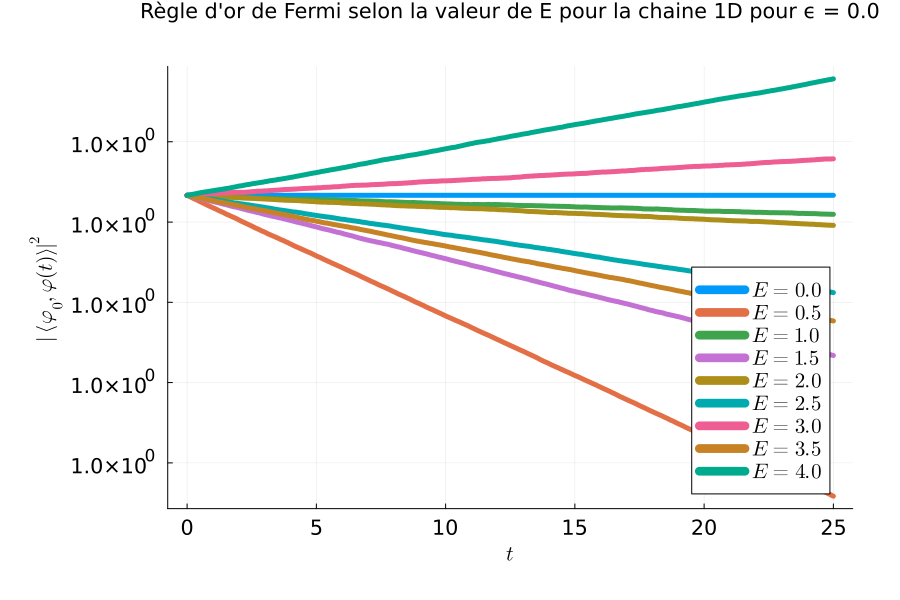
\includegraphics[height=10cm]{Règle d'or de Fermi pour la chaine 1D pour ϵ = 0.png}
        \caption{$\epsilon = 0$}
\end{figure}

En présence d'une perturbation, on remarque que le système quitte l'état propre initial de façon exponentielle avec quelques oscillations, dues à la discrétisation en dimension finie, selon la valeur de la valeur propre initiale $E$. Lorsque $E\in\spec(A)$, il y a décroissance exponentielle : le site et la chaîne peuvent s'échanger de l'information. Dans le cas contraire, les deux systèmes "ne sont pas énergétiquement connectés" et le système reste dans son état initiale avec quelque variations (induites par le $o_\epsilon(1)$. On remarque aussi que le coefficient $\Gamma(\epsilon)$ varie effectivement avec $\epsilon$.

\begin{figure}[h]
    \centering
        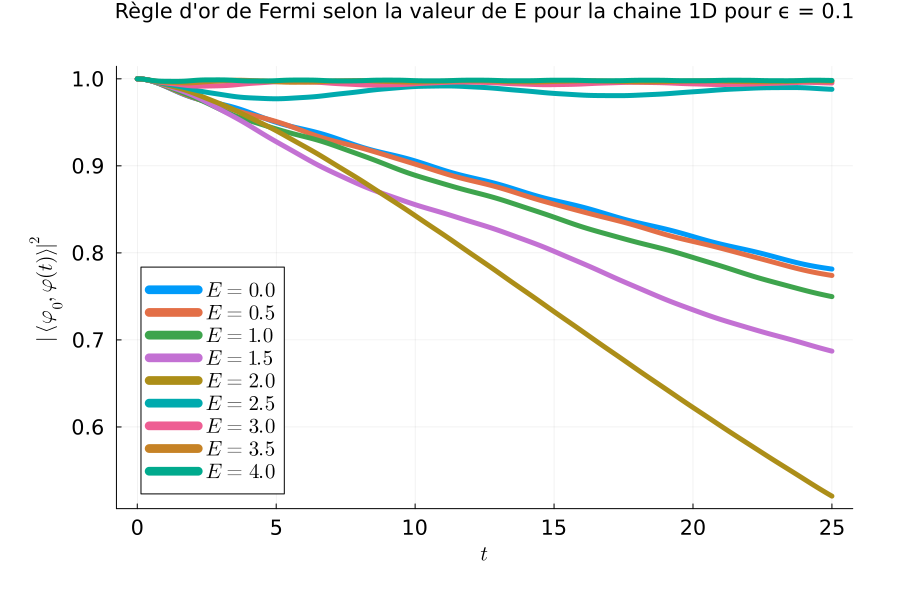
\includegraphics[height=10cm]{Règle d'or de Fermi pour la chaine 1D pour ϵ = 0,1.png}
        \caption{$\epsilon = 0.1$}
\end{figure}

\begin{figure}[h]
    \centering
        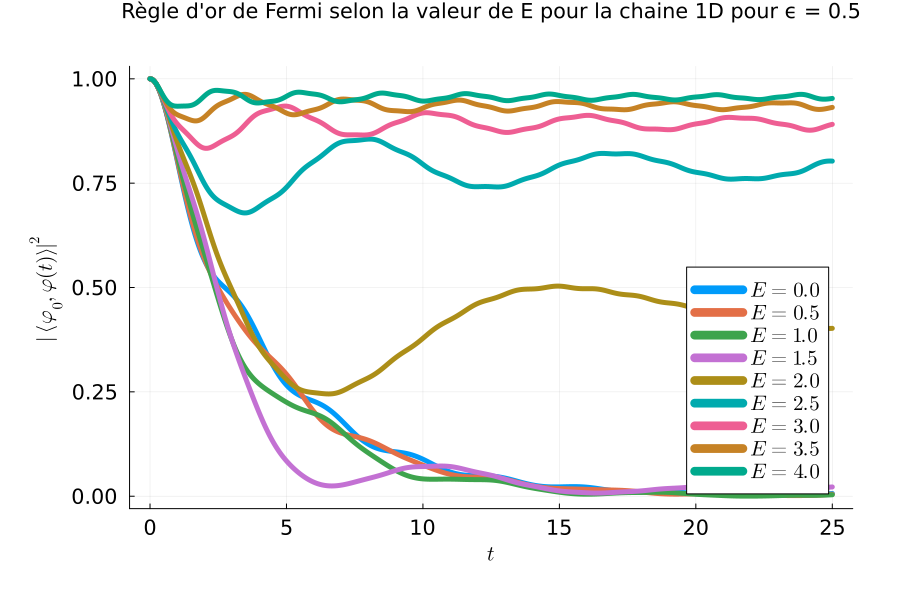
\includegraphics[height=10cm]{Règle d'or de Fermi pour la chaine 1D pour ϵ = 0,5.png}
        \caption{$\epsilon = 0.5$}
\end{figure}
\end{ex}


\mbox{~}
\clearpage
\newpage
\subsection{Objectifs de ce projet}

Comme nous l'avons dit, la règle d'or de Fermi est un résulta bien connue des physiciens. Toutefois, les preuves que l'on peut trouver dans des livres de physiques reposent souvent sur des hypothèses pas toujours claires ou rigoureusement valides. Les mathématiciens, comme souvent, ont cherché à justifier rigoureusement les assertions des physiciens et sont parvenu à établir des résultats sur la règle d'or de Fermi. L'objectif de ce projet est donc d'étudier différentes preuves permettant d'établir la règle d'or de Fermi. Nous investiguerons deux approches très différentes, une dite par les résonances, qui reposent sur de nombreux concepts de théorie spectrale, et sur l'approche de Davies qui repose sur l'étude d'un problème d'évolution. Nous chercherons en particulier à bien expliquer ces preuves et à les clarifier. Nous proposons aussi à étudier un cas particulier de système quantique : le cas de la chaîne 1D connectée à un site, présenté dans la sous-section précédente.


\newpage

\section{Approche par les résonances}

Dans cette partie, nous abordons l'approche dite par les résonances, dénomination que nous expliquerons dans la suite. Pour ce faire, nous commençons par expliquer les grandes lignes de cette approche.
Rappelons les notations. Soit $H(\epsilon)$ un hamiltonien dépendant du paramètre réel positif $\epsilon$ qui est somme d'un hamiltonien initial $H_0$ et d'une perturbation $\epsilon H_1$. On suppose que l'état initial est un vecteur propre $\vp_0$ unitaire $H_0$ associé à une valeur propre $\lambda_0$ de multiplicité finie $m$. Si on note $\mathcal{K}_0$, le sous-espace propre associée, on peut écrire une décomposition de $H(\epsilon)$ dans $\mathcal{K}_0 \oplus \mathcal{K}_0^\perp$ : 
$$H(\epsilon) := 
\underbrace{\begin{pmatrix}
\lambda_0I_m & 0 \\
0    & A 
\end{pmatrix}}_{H_0} \,+\, \epsilon
\underbrace{\begin{pmatrix}
B        & \Gamma \\
\Gamma^* &  C
\end{pmatrix}}_{H_1}$$
où $A$, $B$ et $C$ sont des opérateurs auto-adjoints respectivement de $\mathcal{K}_0^\perp$, $\mathcal{K}_0$ et $\mathcal{K}_0^\perp$, et où $\Gamma$ est une forme linéaire bornée de $\mathcal{K}_0^\perp$ vers $\mathcal{K}_0$.  On notera $E_\epsilon$ la résolution spectrale de $H(\epsilon)$ de sorte que $E_0$ soit la résolution spectrale de $H_0$.

Rappelons aussi que la quantité d'étude qui nous intéresse est la suivante : 
\begin{equation}
    \mid \langle \vp_0 | e^{-iH(\epsilon) t} \vp_0 \rangle\mid^2
\end{equation}
où $t\in\R^+$. L'approche par les résonances consiste à remplacer l'étude de l'exponentielle de l'opérateur $H(\epsilon)$ par l'étude de sa résolvante en utilisant l'information cruciale, portée par $\langle \vp_0 | \cdots |\vp_0 \rangle$,  que l'on regarde le bloc $(\mathcal{K}_0,\mathcal{K}_0)$. Ceci amènera à étudier une résolvante modifiée que nous étudierons dans la sous-section \ref{matrice_livsic}. Les résonances sont en fait les pôles de cette résolvante modifiée. 

Pour ce faire une première idée de comment procéder, regardons le cas lorsqu'il n'y a pas de perturbation, c'est à dire $\epsilon = 0$. Comme $\vp_0$ est un vecteur propre de $H_0$ pour la valeur propre $\lambda_0$, le calcul est immédiat et on trouve 
\begin{equation}
    \mid \langle \vp_0 | e^{-iH_0t} \vp_0 \rangle\mid^2 = |e^{-i\lambda_0t}|^2 = 1.
\end{equation}
Le résultat est logique puisque, en l'absence de perturbation, $\KK_0$ est un sous-espace stable et il n'y a donc aucun moyen d'aller rejoindre d'autres valeurs propres; il y a donc une probabilité $1$ de rester dans le même état. Traité tel quel, le cas sans perturbation ne nous apprend rien de comment traiter le cas avec perturbation. Complexifions alors artificiellement l'approche en faisant apparaître la mesure spectrale de $H_0$. Pour ce faire, il suffit de remarque que $P = E_0(\{\lambda_0\})$ et que $P\vp_0 = \vp_0$, car $\lambda_0$ est une valeur propre de $H_0$. La formule de Stone nous donne alors que 
\begin{eqnarray*}
    \mid \langle \vp_0 | e^{-iH_0t} \vp_0 \rangle\mid^2 &=&\mid \langle \vp_0 | e^{-iH_0t}E_0(\{\lambda_0\}) \vp_0 \rangle\mid^2
    \\ &=& \limeo \mid \langle \vp_0 | \epsilon\im\lp H_0 - \lambda_0 - i\epsilon\rp\inv \vp_0 \rangle\mid^2 \\
    &=& \limeo \mid \langle \vp_0 | \epsilon\im\lp \lambda_0 I_m - \lambda_0 - i\epsilon\rp\inv \vp_0 \rangle\mid^2 \\
    &=&  \limeo \mid \langle \vp_0 | \epsilon\im\lp - i\epsilon\rp\inv \vp_0 \rangle\mid^2\\
    &=&  \mid \langle \vp_0 | \vp_0 \rangle\mid^2 = 1.
\end{eqnarray*}
Pour passer de la deuxième ligne à la troisième ligne, on a utilisé le fait que l'inverse d'un opérateur par bloc est l'opérateur par bloc des inverses. 
Pour généraliser cette approche, on fait face à trois difficultés :
\begin{enumerate}
    \item[1] La difficulté la plus simple à surmonter concerne le passage de la deuxième ligne à la troisième ligne : l'opérateur perturbé n'étant pas diagonal par bloc, il nous faudra étudier quelle est l'expression de sa résolvante sur le bloc $(\KK_0,\KK_0)$, ce que nous faisons ci-après (\ref{matrice_livsic}).
    \item[2] Deuxièmement, si l'information du bloc $(\KK_0,\KK_0)$ pour $H_0$ est concentrée dans la valeur propre $\lambda_0$, sous l'effet de la perturbation, cette valeur propre se modifie et peut se démultiplier en plusieurs valeurs propres de multiplicités inférieures. Pire encore, il peut y avoir de la perte de multiplicité avec une évanescence de la valeur propre vers les valeurs complexes. Ainsi, nous serons amené à regarder la mesure spectrale non pas en $\lambda_0$ mais sur un intervalle $J(\epsilon)$ qui diminue vers le singleton $\{\lambda_0\}$ quand $\epsilon$ tend vers $0$.
    \item[3] Enfin, pour utiliser la formule de Stone, nous devons faire apparaître la mesure spectrale de $H(\epsilon)$ alors que celle qui apparaît naturellement est celle de $H_0$. Pour pallier à ce problème nous aurons recours à des théorèmes dits de concentration spectrale qui forment l'argument principale de la démonstration de la règle d'or de Fermi. En outre ces théorèmes, dont nous donnerons plusieurs versions selon les hypothèses du problème, énoncent que $st-\limeo E_\epsilon(J(\epsilon)) = E_0(\{\lambda_0\}) = P$. Nous verrons cela dans la sous-section $\ref{concentration}$
\end{enumerate}

\subsection{Matrice de Livsic}\label{matrice_livsic}

Nous abordons dans cette partie la notion de matrice de Livsic qui a été introduite en 1957 par M.S Livsic \cite{HOWLAND1975415}, et qui a été redécouvert de nombreuses fois sous différents noms par les physiciens. Il s'agit de la version infini-dimensionnelle de la notion de complément de Schur dont nous ferons un parallèle dans la suite. Considérons un opérateur $H$ auto-adjoint sur un espace de Hilbert $\HH$ de résolution spectrale $E$, $\mathcal{K}_0$ un sous-espace vectoriel de dimension finie de $\HH$, et $P$ la projection orthogonal sur ce sous-espace. La matrice de Livsic est un outil central pour l'approche par les résonances et de façon informel s'agit d'une matrice $B(z)$ dépendant de la variable complexe $z$ qui permet de réécrire la compression $P(H-z)\inv P = (B(z) -z)\inv$. Ainsi, en donnant une formule explicite à cette matrice, nous pourrons étudier de façon explicite le fait que l'on s'intéresse au bloc $(\mathcal{K}_0,\mathcal{K}_0)$ dans la décomposition $\mathcal{K}_0\oplus \mathcal{K}_0^\perp$ de la résolvante de $H$.

Faisons un petit rappel sur la résolvante notée $R(z) := (H-z)\inv$. Cette quantité est bien définie sur le complémentaire du spectre de $H$ et y est holomorphe. A l'instar des différents types de singularités en analyse complexe, cette quantité est méromorphe sur une certaine partie du spectre : le spectre discret. Pour rappel, le spectre discret $\sigma_d(H)$ est l'ensemble des valeurs propres de multiplicité finie de $H$. La résolvante est donc méromorphe sur le complémentaire du spectre essentiel $\sigma_{ess}(H) = \sigma(H)\setminus\sigma_d (H)$. La compression $PR(z)P$ est donc aussi méromorhpe sur  $\C\setminus\sigma_{ess}(H)$.

Commençons par établir l'existence d'une telle matrice $B(z)$. Celle-ci repose sur le faire que la compression $PR(z)P$ est un opérateur de dimension finie, i.e une matrice, et la proposition suivante.

\begin{prop}
    $PR(z)P$ est inversible pour $z\in\C\setminus\R$.
\end{prop}
\begin{proof}
    D'après la remarque précédente, il suffit donc de montrer que cette quantité est injective. Soit $z = a+ib\in\C\setminus\R$ et $x\in \mathcal{K}_0$ tel que $PR(z)Px = 0$. En particulier, on a 

    $$0 = \im\la x\,,\, PR(z)Px \ra = \im\la x\,,\, R(z)x \ra = b\lb\lb\lp (H-a)^2 + b^2 \rp^{-1/2}x\rb\rb^2$$
    car $x = Px$, et car $P$ et $H$ sont auto-adjoint. Comme $b$ est non nul, nécessairement $x = 0$.
\end{proof}

Cela nous permet de définir la notion de matrice de Livsic.

\begin{Def}[Matrice de Livsic]
Pour $z\in \C\setminus\R$, on définit la matrice de Livsic sur $\mathcal{K}_0$ par
\begin{equation*}
    B(z) := (PR(z)P)\inv + z
\end{equation*}
qui vérifie l'identité 
\begin{equation*}
    (B(z)-z)\inv = P(H-z)\inv P.
\end{equation*}
Cet identité nous permet d'étendre la définition de $B(z)$ sur $\C\setminus\sigma_{ess}(H)$.
\end{Def}

\begin{rem}
    La dénomination \textit{matrice} de Livsic est bien choisie car l'opérateur $B(z)$ est bien un endomorphisme linéaire d'un espace vectoriel de dimension finie, $\mathcal{K}_0$, pour tout $z\in\C\setminus\sigma_{ess}(H)$.
\end{rem}

La connaissance de l'existence d'une telle matrice $B(z)$ n'est pas très utile en soi, et une expression explicite en fonction de $z$, de $P$ et de $H$ serait plus intéressante. Pour ce faire quelques idées, nous allons d'abord analyser le cas où $\dim \HH < +\infty$ dans le paragraphe suivant. 

\paragraph{Complément de Schur}
Cette notion de matrice de Livsic fait écho avec sa version finie dimensionnelle bien connue : le complément de Schur.  
Soient $n,m \in\N^*$. Considérons une matrice $A\in\C^{(n+m)\times (n+m)}$ hermitienne s'écrivant 
\begin{equation*}
    A:= \begin{pmatrix}
A_{11} & A_{12} \\
A_{21} & A_{22} 
\end{pmatrix}
\end{equation*}
avec $A_{11}\in\R^{n\times n},  A_{12}\in\C^{n\times m}, A_{21}\in\C^{m\times n}$ et $A_{22}\in\C^{m\times m}$. Soit $\lambda \in \R$ et cherchons à résoudre le problème aux valeurs propres $Ax = \lambda x$ d'inconnue $x\in\R^{n+m}$ en supposant que $\lambda$ ne soit pas valeur propre de $A_{22}$. La deuxième ligne de ce système conduit à l'égalité $x_2 = -(A_{22}-\lambda)^{-1}A_{21}x_1$ que l'on peut injecter dans la première ligne et obtenir $(A_{11} - A_{12}(A_{22}-\lambda)^{-1}A_{21})x_1 = \lambda x_1 $. On obtient donc $\lp A_{11} - A_{12}(A_{22}-\lambda)^{-1}A_{21} - \lambda  \rp^{-1} x_1 = 0$. Autrement dit le complément de Schur, ou encore la matrice de Livsic, s'écrit : $A_{11} - A_{12}(A_{22}-\lambda)A_{21}$. 

\begin{rem}
Faisons quelques remarques à la lueur du cas fini-dimensionnel précédent :
\begin{enumerate}
    \item Une remarque importante qui doit être faite est que la matrice de Livsic est un outil qui permet de réduire la dimension du problème. Par exemple, dans le cas fini-dimensionnel précédent, nous sommes passés d'un problème aux valeurs propres de dimension $n+m$ à un problème de dimension $n$.
    \item On remarque aussi que $\lambda$ est valeur propre de $A$ si et seulement si $\lambda$ est valeur propre de la matrice de Livsic car sinon, dans le calcul précédent, on aurait que $x_1 = 0$ et par la relation précédente $x_2 = 0$.
\end{enumerate}
 
Nous allons maintenant chercher à obtenir des résultats similaires dans le cas général. Écrivons $H$ dans la décomposition $\HH = \mathcal{K}_0 \oplus \mathcal{K}_0^\perp$ :
\begin{equation}
    H = \begin{pmatrix}
        T & \Gamma \\
        \Gamma^* & A 
\end{pmatrix}
\end{equation}
où $\Gamma$ est une application linéaire de $\mathcal{K}_0^\perp$ dans $\mathcal{K}_0$, $A$ et $T$ sont des opérateurs auto-adjoints respectivement de $\mathcal{K}_0^\perp$ et de $\mathcal{K}_0$. Autrement dit, on a $T = PHP$, $\Gamma = PH(I-P)$ et $A = (I-P)H(I-P)$. On notera parfois $P^\perp = I - P$.

\begin{prop}[Formule explicite de la matrice de Livsic]\label{formulue_liv}
Pour tout $z\in\C\setminus\sigma_{ess}(H)$, on a 
\begin{equation}
    B(z) = T - \Gamma(A -z)^{-1}\Gamma^*
\end{equation}
\end{prop}

\begin{proof}
    Décomposons $H$ comme somme de deux opérateurs $H = D + V$ où $D = T\oplus A$ et $V = \Gamma + \Gamma^*$. Soit $Z \in\C\setminus\sigma(H)$. Par la seconde formule de la résolvante [], on a :
    \begin{equation}
        (H-z)^{-1} = (D-z)^{-1} - (D-z)^{-1}V(D-z)^{-1} + (D-z)^{-1}V(D-z)^{-1}V(H-z)^{-1}.
    \end{equation}
    On peut ensuite compresser sur $E_0$, en utilisant le fait que l'opérateur $D$ est diagonal dans la décomposition $\mathcal{K}_0 \oplus \mathcal{K}_0^\perp$ :
    \begin{eqnarray}
        P(H-z)^{-1}P &=&  (T-z)^{-1} - (T-z)^{-1}PVP(T-z)^{-1} \\
        & & + \, (T-z)^{-1}\Gamma P^\perp (D-z)^{-1} P^\perp \Gamma^* P(H-z)^{-1}P \\
        & = & (T-z)^{-1} + (T-z)^{-1}\Gamma (A-z)^{-1}  \Gamma^* P(H-z)^{-1}P
    \end{eqnarray}
    Cela donne une équation en $P(H-z)^{-1}P$ que l'on peut isoler pour donner :
    \begin{eqnarray}
        P(H-z)^{-1}P &=& \lp I -   (T-z)^{-1}\Gamma (A-z)^{-1}  \Gamma^*\rp^{-1} (T-z)^{-1} \\
        &=& \lp T -\Gamma^*(A-z)^{-1}\Gamma - z\rp^{-1},
    \end{eqnarray}
    ce qui démontre le résultat.
\end{proof}

\begin{ex}
    Pour le cas qui nous intéresse en particulier, nous avons $B(\epsilon,z) = E - \epsilon^2 e_{R_0}^*(A-z)\inv e_{R_0}$ qui est un scalaire complexe.
\end{ex}

Le lien entre les valeurs propres de $B(z)$ et celles de $H$ est donné dans la proposition suivante. Pour ce faire, nous donnons d'abord la définition suivante :
\begin{Def}
    Un sous-espace vectoriel $\mathcal{K}$ de $\HH$ est dit cyclique si le plus petit sous-espace stable de $\HH$ tel que l'orthogonal soit soit aussi stable et qui contient $\mathcal{K}$ est exactement $\mathcal{K}$. 
\end{Def}

Donnons maintenant la proposition dont la preuve peut être trouvée dans \cite{HOWLAND1975415}.

\begin{prop}[Lien entre valeur propre de $H$ et de $B(z)$]\label{link_vp}
Si $\mathcal{K}_0$ est cyclique alors tous zéros de $z\in \C\setminus \sigma_{ess}(H) \mapsto \det \lp B(z) -z \rp$ de multiplicité $m$ est une valeur propre de $H$ de même multiplicité.
\end{prop}

Enfin terminons avec un résultat important qui va nous servir pour démontrer la règle d'or de Fermi : il s'agit de la formule de Stone "version" matrice de Livsic. Celle-ci nous sera utile pour procéder de manière similaire au cas simple de l'introduction de cette section.

\begin{prop}[Formule de Stone]\label{Stones_Liv}
    Supposons que $z\in\C\setminus\R \mapsto B(z)$ possède une extension sur un intervalle réel $I$ que l'on note $B(\lambda)$ pour $\lambda\in I$. Comme pour la formule de Stones classique, il y a en fait deux formules selon le cas :
    \begin{enumerate}
        \item Soit $J\subseteq I$ et supposons qu'aucun élément $\lambda$ de $J$ ne soit valeur propre de $B(\lambda)$. On a alors
        \begin{equation}
            PE(J)P = \f{1}{\pi}\int_J (B(\lambda) - \lambda)^{-1}\dd \lambda.
        \end{equation}
        \item Si $\lambda \in I$ est une valeur propre de $B(\lambda)$ alors
        \begin{equation}
            PE(\{ \lambda \})P = st-\lim\limits_{\epsilon \rightarrow 0^+} \epsilon \im \lp B(\lambda + i\epsilon  )- \lambda - i\epsilon\rp ^{-1}.
        \end{equation}
    \end{enumerate}
\end{prop}
Ces formules sont très similaires aux formules de Stones classique et intègrent bien le fait que l'on se concentre sur le bloc $(\mathcal{K}_0,\mathcal{K}_0)$.

\begin{proof}
    Pour la première formule, l'hypothèse permet d'appliquer confortablement la formule de Stone à l'opérateur $H$ et il suffit de compresser par $P$ qui commute avec l'intégrale.
    Pour la deuxième, il faut remarquer que le projecteur $P$ est continue par rapport à la limite forte pour le faire commuter avec la limite.
\end{proof}


\subsection{Théorèmes de concentration spectrale}\label{concentration}

Nous passons maintenant au théorème de concentration spectrale. Nous allons en fait en voir plusieurs versions avec des hypothèses différents, mais qui vont aboutir au même résultat. Comme expliquer dans l'introduction de cette section, le but est de pouvoir substituer le projecteur $P$ sur le sous-espace propre $\mathcal{K}_0$ associé à la valeur propre $\lambda_0$ par la résolution spectrale $E_\epsilon$ de l'hamiltonien perturbé $H(\epsilon)$ évalué sur un certain ensemble $J(\epsilon)$ avec une erreur en $o(1)$ en $\epsilon \rightarrow 0^+$.

Intuitivement, il faut comprendre ceci. On sait que $\lambda_0$ est une valeur propre de $H_0$ et de la matrice de Livsic associée qui est $B(z,0) = \lambda_0 I_m$, où on rappelle que $m = \dim \mathcal{K}_0$. Pour étudier l'effet de la perturbation sur cette valeur propre, en accord avec le théorème \ref{link_vp}, il convient d'étudier l'évolution des zéros de l'équation$\det (B(z,\epsilon) - z) = 0$ avec $\epsilon$. Si initialement pour $\epsilon = 0$ il y a un unique zéros, $\lambda_0$, de multiplicité $m$, celui va possiblement se séparer en plusieurs zéros dont la somme des multiplicités restent $m$, et se déplacer de façon continue avec $\epsilon$. Le point important à noter est que la matrice de Livsic n'est généralement pas auto-adjointe, ou en d'autres termes hermitiennes, ce qui implique que les zéros de  $\det (B(z,\epsilon) - z) = 0$ ne sont plus nécessairement réels.

\begin{figure}
\centering


\tikzset{every picture/.style={line width=0.75pt}} %set default line width to 0.75pt        

\begin{tikzpicture}[x=0.75pt,y=0.75pt,yscale=-1,xscale=1]
%uncomment if require: \path (0,221); %set diagram left start at 0, and has height of 221

%Straight Lines [id:da47644697694222793] 
\draw [line width=1.5]    (136,106.35) -- (583,106.95) ;
\draw [shift={(586,106.95)}, rotate = 180.08] [color={rgb, 255:red, 0; green, 0; blue, 0 }  ][line width=1.5]    (14.21,-4.28) .. controls (9.04,-1.82) and (4.3,-0.39) .. (0,0) .. controls (4.3,0.39) and (9.04,1.82) .. (14.21,4.28)   ;
\draw  [line width=1.5]  (323.33,86.34) -- (358.72,126.53)(358.72,86.34) -- (323.33,126.53) ;
\draw  [line width=1.5]  (416.54,1.6) -- (434.23,21.69)(434.23,1.6) -- (416.54,21.69) ;
\draw  [line width=1.5]  (232.56,96.32) -- (250.26,116.42)(250.26,96.32) -- (232.56,116.42) ;
\draw  [line width=1.5]  (382.7,190.51) -- (400.39,210.6)(400.39,190.51) -- (382.7,210.6) ;
%Curve Lines [id:da3347968015604388] 
\draw [line width=1.5]  [dash pattern={on 1.69pt off 2.76pt}]  (341.17,98.16) .. controls (359.01,32.58) and (356.97,35.33) .. (409.74,13.7) ;
\draw [shift={(412.19,12.69)}, rotate = 157.65] [color={rgb, 255:red, 0; green, 0; blue, 0 }  ][line width=1.5]    (14.21,-4.28) .. controls (9.04,-1.82) and (4.3,-0.39) .. (0,0) .. controls (4.3,0.39) and (9.04,1.82) .. (14.21,4.28)   ;
%Curve Lines [id:da3982201365980109] 
\draw [line width=1.5]  [dash pattern={on 1.69pt off 2.76pt}]  (350.22,107.73) .. controls (387.86,107.73) and (398.53,151.88) .. (390.64,189.7) ;
\draw [shift={(390,192.6)}, rotate = 283.26] [color={rgb, 255:red, 0; green, 0; blue, 0 }  ][line width=1.5]    (14.21,-4.28) .. controls (9.04,-1.82) and (4.3,-0.39) .. (0,0) .. controls (4.3,0.39) and (9.04,1.82) .. (14.21,4.28)   ;
%Curve Lines [id:da3997073011772787] 
\draw [line width=1.5]  [dash pattern={on 1.69pt off 2.76pt}]  (339.74,103.57) .. controls (312.46,97.06) and (282.04,96.86) .. (251.1,102.79) ;
\draw [shift={(248.23,103.35)}, rotate = 348.5] [color={rgb, 255:red, 0; green, 0; blue, 0 }  ][line width=1.5]    (14.21,-4.28) .. controls (9.04,-1.82) and (4.3,-0.39) .. (0,0) .. controls (4.3,0.39) and (9.04,1.82) .. (14.21,4.28)   ;

% Text Node
\draw (332.22,137.93) node [anchor=north west][inner sep=0.75pt]   [align=left] {$\displaystyle \lambda _{0}$};
% Text Node
\draw (442.06,11.49) node [anchor=north west][inner sep=0.75pt]  [font=\footnotesize] [align=left] {$\displaystyle \xi _{1}( \epsilon )$};
% Text Node
\draw (406.39,197.63) node [anchor=north west][inner sep=0.75pt]  [font=\footnotesize] [align=left] {$\displaystyle \xi _{2}( \epsilon )$};
% Text Node
\draw (222.46,73.76) node [anchor=north west][inner sep=0.75pt]  [font=\footnotesize] [align=left] {$\displaystyle \xi _{3}( \epsilon )$};
% Text Node
\draw (334,117.11) node [anchor=north west][inner sep=0.75pt]   [align=left] {$\displaystyle m$};
% Text Node
\draw (294.91,81.39) node [anchor=north west][inner sep=0.75pt]  [font=\footnotesize] [align=left] {$\displaystyle m_{3}$};
% Text Node
\draw (401.91,143.91) node [anchor=north west][inner sep=0.75pt]  [font=\footnotesize] [align=left] {$\displaystyle m_{2}$};
% Text Node
\draw (363.44,43.32) node [anchor=north west][inner sep=0.75pt]  [font=\footnotesize] [align=left] {$\displaystyle m_{1}$};
% Text Node
\draw (187.91,171.91) node [anchor=north west][inner sep=0.75pt]  [font=\normalsize] [align=left] {$\displaystyle m\ =\ m_{1} +m_{2} +m_{3}$};


\end{tikzpicture}

\caption{Illustation de la séparation de la valeur propre initialle}
\end{figure}


Prenons maintenant $m = 1$ pour simplifier. Dans ce cas, le zéro initial $\lambda_0$ se déplace simplement dans le plan complexe $\lambda(\epsilon)$, sans effet de séparation.  Il y a deux cas de figure :
\begin{enumerate}
    \item Soit sur un voisinage $U$ de $0$ pour $\epsilon$,  $\lambda(\epsilon)$ est réel. Dans ce cas $\lambda(\epsilon)$ est une valeur propre de $H(\epsilon)$ et la théorie classique des perturbations dit que l'état propre $\vp_0$ dans lequel on se trouve subit une perturbation continue $\vp(\epsilon)$ en restant un état propre de $H(\epsilon)$. En d'autres termes,  
    toute "l'information" portée par $\lambda_0$ est transportée vers $\lambda(\epsilon)$. Pour récupérer cette information, il semble alors naturel que $P=E_0\lp\{\lambda_0\}\rp$ se déplace vers $E_\epsilon\lp\{\lambda(\epsilon)\}\rp$.  
    \item Soit sur un voisinage $U$ de $0$ pour $\epsilon$, $\lambda(\epsilon)$ est complexe non réel. Dans ce cas, il y a une perte d'information car $\lambda(\epsilon)$ n'étant plus réel ne pourra plus être une valeur propre de $H(\epsilon)$ et donc être le siège d'informations. Ainsi, on ne peut plus considérer $E_\epsilon\lp\{\lambda(\epsilon)\}\rp$ car cette quantité sera systématiquement égal à $0$, mais à la place il faut évaluer la résolution spectrale $E_\epsilon$ en un intervalle $J(\epsilon)$, à l'instar des éléments du spectre non ponctuel. Il semble aussi naturel de choisir un intervalle centré en la partie réel de $\lambda(\epsilon)$. Notons $J(\epsilon) = [\lambda(\epsilon)-\delta(\epsilon),\lambda(\epsilon)+\delta(\epsilon)]$. Quant à l'évolution des bornes, il faut faire attention à ce que la partie complexe de $\lambda(\epsilon)$ est le temps de rejoindre son point d'origine $\lambda_0$ avant que les bornes $\delta(\epsilon)$ ne s'annulent. Cela conduira à prendre au moins la condition suivante : $\im(\lambda(\epsilon)) = o(\delta(\epsilon)$. C'est un moyen qu'à l'échelle de l'intervalle, on ne "voit" pas la partie imaginaire de $\lambda(\epsilon)$ et donc la perte d'information.
\end{enumerate}



\begin{figure}[h]
    \centering
\begin{tikzpicture}[x=0.75pt,y=0.75pt,yscale=-1,xscale=1]
%uncomment if require: \path (0,221); %set diagram left start at 0, and has height of 221
%Straight Lines [id:da807849214616583] 
\draw [line width=1.5]    (157.2,106.75) -- (341.2,107.24) ;
\draw [shift={(344.2,107.25)}, rotate = 180.15] [color={rgb, 255:red, 0; green, 0; blue, 0 }  ][line width=1.5]    (14.21,-4.28) .. controls (9.04,-1.82) and (4.3,-0.39) .. (0,0) .. controls (4.3,0.39) and (9.04,1.82) .. (14.21,4.28)   ;
\draw  [line width=1.5]  (299.6,96.84) -- (317.31,116.95)(317.38,96.76) -- (299.52,117.03) ;
\draw  [line width=1.5]  (217.48,31.91) -- (235.18,52.01)(235.26,31.82) -- (217.4,52.1) ;
%Curve Lines [id:da2367878250500588] 
\draw [line width=1.5]  [dash pattern={on 1.69pt off 2.76pt}]  (304.74,106.07) .. controls (277.06,63.56) and (264.46,50.06) .. (234.98,41.98) ;
\draw [shift={(232.2,41.25)}, rotate = 14.25] [color={rgb, 255:red, 0; green, 0; blue, 0 }  ][line width=1.5]    (14.21,-4.28) .. controls (9.04,-1.82) and (4.3,-0.39) .. (0,0) .. controls (4.3,0.39) and (9.04,1.82) .. (14.21,4.28)   ;
%Straight Lines [id:da927739341142745] 
\draw [line width=1.5]  [dash pattern={on 1.69pt off 2.76pt}]  (226.2,46.75) -- (226.2,104.75) ;
%Straight Lines [id:da4326288412728301] 
\draw [color={rgb, 255:red, 255; green, 0; blue, 33 }  ,draw opacity=1 ][fill={rgb, 255:red, 251; green, 8; blue, 36 }  ,fill opacity=1 ][line width=2.25]    (187.7,106.75) -- (262.2,106.75) ;
%Straight Lines [id:da8393744285522509] 
\draw [line width=1.5]    (400.2,106.25) -- (584.2,106.74) ;
\draw [shift={(587.2,106.75)}, rotate = 180.15] [color={rgb, 255:red, 0; green, 0; blue, 0 }  ][line width=1.5]    (14.21,-4.28) .. controls (9.04,-1.82) and (4.3,-0.39) .. (0,0) .. controls (4.3,0.39) and (9.04,1.82) .. (14.21,4.28)   ;
\draw  [line width=1.5]  (542.6,96.34) -- (560.31,116.45)(560.38,96.26) -- (542.52,116.53) ;
\draw  [line width=1.5]  (539.48,96.41) -- (557.18,116.51)(557.26,96.32) -- (539.4,116.6) ;
%Straight Lines [id:da14976654521532762] 
\draw [color={rgb, 255:red, 255; green, 0; blue, 33 }  ,draw opacity=1 ][fill={rgb, 255:red, 251; green, 8; blue, 36 }  ,fill opacity=1 ][line width=2.25]    (521.8,106.75) -- (570.2,107.25) ;

% Text Node
\draw (300.22,119.93) node [anchor=north west][inner sep=0.75pt]   [align=left] {$\displaystyle \lambda _{0}$};
% Text Node
\draw (189.96,30.76) node [anchor=north west][inner sep=0.75pt]  [font=\footnotesize] [align=left] {$\displaystyle \xi ( \epsilon )$};
% Text Node
\draw (213.96,111.26) node [anchor=north west][inner sep=0.75pt]  [font=\footnotesize] [align=left] {$\displaystyle \lambda ( \epsilon )$};
% Text Node
\draw (191.96,67.76) node [anchor=north west][inner sep=0.75pt]  [font=\footnotesize] [align=left] {$\displaystyle \Gamma ( \epsilon )$};
% Text Node
\draw (230.46,84.76) node [anchor=north west][inner sep=0.75pt]  [font=\footnotesize] [align=left] {$\displaystyle \textcolor[rgb]{0.94,0.03,0.14}{J( \epsilon )}$};
% Text Node
\draw (558.22,111.93) node [anchor=north west][inner sep=0.75pt]   [align=left] {$\displaystyle \lambda _{0}$};
% Text Node
\draw (525.46,117.76) node [anchor=north west][inner sep=0.75pt]  [font=\footnotesize] [align=left] {$\displaystyle \lambda ( \epsilon )$};
\end{tikzpicture}
    \caption{Illustration de l'intervalle $J(\epsilon)$ et de son comportement asymptotique quand $\epsilon \rightarrow 0^+$}
    \label{fig:enter-label}
\end{figure}      



\subsubsection{Version de Howland}

Dans son article intitulé \textit{The Livsic  Matrix in Perturbation Theory}  (\cite{HOWLAND1975415}), James S. Howland propose en 1975 un théorème de concentration spectrale intéressant, sous l'hypothèse relativement forte mais qui est souvent vérifiée : la possibilité d'effectuer un certain prolongement analytique de la matrice de Livisc du plan complexe supérieur vers le plan complexe inférieur.

Rappelons d'abord la définition suivante :
\begin{Def}[Convergence forte (généralisée) d'opérateurs]
\,
    \begin{enumerate}
        \item Une suite d'opérateurs $(A_n)\in\mathcal{L}(\HH)^\N$ converge fortement vers l'opérateur $H\in\mathcal{L}(\HH)$ si $\forall u\in \HH$, on a
        $\lim\limits_{n\rightarrow +\infty} A_n u = Au$.
        \item Une suite d'opérateurs $(A_n)$ converge fortement vers l'opérateur $A$ dans le sens généralisé si la suite des résolvantes $(R_n)$ de la suite $(A_n)$ converge fortement vers la résolvante de $A$.
    \end{enumerate}
\end{Def}

Passons maintenant au théorème de Howland. Nous donnons une preuve plus détaillée que celle se trouvant dans \cite{HOWLAND1975415}.

\begin{theo}[\textbf{Concentration spectrale - Howland (1975)}]
\,

Supposons que \begin{enumerate}
    \item[(1)] pour tout $n\in\N$, $B(\epsilon,z)$ possède un prolongement analytique toujours noté $B(\epsilon,z)$ du plan complexe supérieur sur un voisinage $ \Omega$ de $\lambda_0$,
    \item[(2)] $\lp B(\epsilon,z)\rp$ converge fortement vers $B(z)$ uniformément sur $\Omega$.
\end{enumerate}
Alors, pour $\epsilon$ assez petit, l'équation sur $z$ : $\det(B(\epsilon,z) -z) = 0 $ possède exactement $m$ solutions comptées avec multiplicités dans $\Omega$. De plus, si on note $\xi_k(\epsilon) = \lambda_k(\epsilon) - i \Gamma_k(\epsilon)$ pour $k\in\{1,\cdots,m\}$ ces solutions, et si on choisis une suite $(\delta_k(\epsilon))$ de réels positifs de sorte que $\Gamma_k(\epsilon) = o(\delta_k(\epsilon))$, alors en définissant les intervalles 
$$ J(\epsilon) = \bigcup_{k=1}^m (\lambda_k(\epsilon) - \delta_k(\epsilon),\lambda_k(\epsilon) + \delta_k(\epsilon))$$ alors $P = st-\lim\limits_{\epsilon\rightarrow 0^+} E_\epsilon(J(\epsilon))$.
\end{theo}

\begin{proof}
\underline{Étape 1} : Commençons par prouver l'existence des zéros. Par hypothèse, on a que la suite de matrices $(B_n(z))$ converge uniformément sur $\Omega$ vers $B(z)$, ce qui implique, en combinant au fait que le déterminant est continue, que pour $n$ assez grand et tout $z\in\Omega$, $$ |\det (B_n^+(z) - z) - \det (B(z) - z)| < \epsilon = |\det (B(z) - z)| $$ car $|B_n^+(z) - z - (B(z) - z)| \leq ||B_n - B|| \rightarrow 0$. Ceci étant vrai pour tout $z\in\Omega$, ceci est vrai pour tout $z\in\gamma$ où $\gamma$ est un chemin inclus dans $\Omega$ et entourant $\lambda_0$. Comme $\lambda_0$ est l'unique zéro et de multiplicité $m$ de $\det (B(z) - z)$, par théorème de Rouché, l'équation $\det(B_n^+(z) -z) = 0$ a exactement $m$ solutions comptées avec multiplicité. 

\underline{Étape 2} : Montrons maintenant que $\lim\limits_{n\rightarrow +\infty} E_n(J_n) Px = Px$ for $x\in\HH$.



\underline{Étape 3} : Enfin, il reste à montrer que $\lim\limits_{n\rightarrow +\infty} E_n(J_n) (I-P)x = 0$ for $x\in\HH$. Pour ce faire, il faut remarquer que $\forall k\in \{1,\cdots,m\}, \lim\limits_{n\rightarrow +\infty}\lambda_k(n) = \lambda_0$ car si $\psi$ est un vecteur propre de $B_n(z)$ alors $\lambda_k(n) \psi = B_n(z)\psi \rightarrow B(z) \psi = \lambda_0 \psi$. Ainsi, pour $\epsilon >0$, il existe un certain rang $N$ tel que $\forall n\geq N$, 
\begin{equation}
    J(n) \subseteq (\lambda_0 - \epsilon, \lambda_0 + \epsilon)
\end{equation}
\end{proof}

\begin{rem}[\textbf{Cas des matrices dans un cas particulier de la théorie de la diffusion}]
Supposons que nous avons une matrice hermitienne $H(\kappa)$ dépendant d'un paramètre $\kappa \geq 0$ définie par $$H(\kappa) := 
\underbrace{\begin{pmatrix}
\lambda_0 I_m & 0 \\
0    & A 
\end{pmatrix}}_{H_0} + \kappa
\underbrace{\begin{pmatrix}
0        & \Gamma^* \\
\Gamma &  0
\end{pmatrix}}_{H_1}$$ où $\lambda_0\in\R$, $m\geq 1$ un entier, $A$ est une matrice hermitienne n'ayant pas $\lambda_0$ comme valeur propre, $\Gamma$ une matrice non nécessairement carré et $I_m$ l'identité des matrices de taille $m$. $\lambda_0$ est clairement une valeur propre de $H_0$ de multiplicité $m$ et $\lim\limits_{\kappa\rightarrow 0} H(\kappa) = H_0$, sous n'importe quel sens, les normes étant toutes équivalentes en dimension finie. La matrice de Livisc de $H(\kappa)$ est $B(\kappa,z) = \lambda_0I_m - \kappa^2\Gamma^* (A-z)^{-1} \Gamma$. Il est clair que la matrice précédente possède un prolongement méromorphe sur $\C\backslash \spec(A)$. En effet, on peut clairement voir que $(A-z)^{-1}$ est méromorphe sur $\C\backslash \spec(A)$ par la formule qui la relie au cofacteur de $A$. En particulier, comme $\spec(A)\cap \{\lambda_0\} = \emptyset$, $B(\kappa,z)$ possède un prolongement analytique sur un voisinage de $\lambda_0$. Comme ce prolongement a la même expression, le point (2) du théorème précédent est directement vérifié. De plus $B(\kappa,z)$ est une matrice hermitienne de taille $m$, elle possède $m$ valeurs propres réelles. Le théorème précédent affirme que si $\kappa$ est suffisamment petit elles sont dans un voisinage de $\lambda_0$ choisit, ce qui peut aussi se voir par le fait que $B(z,\kappa)$ est polynomiale en $\kappa$. Dans le théorème précédent, tous les $\Gamma_k(\kappa)$ sont nuls et on peut prendre $\delta_k(\kappa) = 0$ pour tout $\kappa\geq 0$ et $k\in\{1,\cdots,m\}$. En notant $|\lambda_k(\kappa)\rangle$ un vecteur propre unitaire associé à $\lambda_k(\kappa)$ (et tels que les $|\lambda_k(\kappa)\rangle$ forment une base de $\R^m$), on obtient le résultat classique de théorie des perturbations:
$$st-\lim\limits_{\kappa\rightarrow 0} \sum_{k=1}^m  \lambda_k(\kappa)|\lambda_k(\kappa)\rangle \langle\lambda_k(\kappa)| = \lambda_0|\lambda_0\rangle\langle\lambda_0|.$$
\end{rem}

\subsubsection{Version de Orth}

Nous nous sommes ensuite intéressé à un autre théorème de concentration spectrale, présenté dans l'article \cite{Orth1990} \textit{Quantum Mechanical Resonance
 and Limiting Absorption: The Many Body Problem} proposé par Orth en 1990. Il a pour but de préciser d'autres hypothèses suffisantes pour établir le théorème de concentration spectrale que le théorème de Howland avec des hypothèses ne couvre pas. Ici il n'y a plus d'hypothèse de prolongement analytique, mais on suppose de la lipschitziannité de certains termes. Cela amène à donner une définition différente, plus large, de ce qu'est une résonance dans ce contexte de mécanique quantique. En effet, puisque l'on ne parle plus de prolongement analytique, il est plus délicat de parles des pôles de la résolvante et d'une matrice de Livsic associée.
 
 Nous reprenons les notations de l'introduction de cette section. Pour des raisons techniques, nous allons nous concentrer sur le cas particulier où $\dim \mathcal{K}_0 = 1$. 

 \begin{Def}[Résonances simple]
     Supposons $\dim \mathcal{K}_0 = 1$. On dira que la famille d'opérateur $(H(\epsilon))_{\epsilon \geq 0}$ possède une résonance en $\lambda_0\in\R^*$ s'il existe
     \begin{enumerate}
         \item un voisinage réel $I$ de $\lambda_0$,
         \item un voisinage réel $U$ de $0$,
         \item un sous-espace vectoriel $\mathcal{H}^+$ dense de $\mathcal{H}$ dont le dual est noté $\mathcal{H}^-$,
     \end{enumerate}
     tels que
     \begin{enumerate}
         \item[a)] $\forall \epsilon\in U$, $z\in\C\setminus\R \mapsto \lp P^\perp H(\epsilon)P^\perp - z\rp^{-1}$ se prolonge sur $I$ comme opérateur borné de $\mathcal{H}^+$ vers $\mathcal{H}^-$. Ce prolongement est lipschitz continue de constante $L(\epsilon) = o(\epsilon^{-2})$,
         \item[b)] $\mathcal{K}_0 \subseteq \mathcal{H}^+$ et $H_1(\mathcal{K}_0) \subseteq \mathcal{K}_0$,
         \item[c)] $\forall \epsilon \in U$, et pour toute valeurs propres (il peut ne pas y en avoir) $\mu(\epsilon) \in I$ de $H(\epsilon)$ le vecteur propre associé est dans $\mathcal{H}^+$.
     \end{enumerate}
 \end{Def}

Expliquons un peu cette définition de résonance et pourquoi de telles hypothèses. L'hypothèse de prendre un voisinage $I$ de $\lambda_0$ et de regarder un certain prolongement autour de $I$ est assez logique car on va perturber légèrement le système qui se trouve initialement en $\lambda_0$. Il est aussi logique de considérer un voisinage $U$ de $0$ car on s'intéresse à une limite en $0$ de la perturbation d'amplitude $\epsilon$. Passons à moins évident : le fait de regarder un sous-espace vectoriel $\mathcal{H}^+$ dense de $\mathcal{H}$ au lieu de tout simplement $\mathcal{H}$. En fait, cela vient du fait que l'on souhaite à prolonger de façon continue (et même Lipschitz) la résolvante du bloc $(\mathcal{K}_0^\perp,\mathcal{K}_0^\perp)$ de l'hamiltonien perturbé. Pour avoir cette prolongation, il faut ne pas intersecter le spectre de $H(\epsilon)$, ce qui pourrait être un problème. En effet, puisque $\lambda_0$ n'est pas une valeur propre de $P^\perp H_0 P^\perp$, il en est de même de $\lambda(\epsilon)$ vis à vis de $P^\perp H(\epsilon)P^\perp$ pour $\epsilon$ suffisamment petit. Cependant $\lambda(\epsilon)$ peut tout à fait appartenir au spectre non ponctuel de $P^\perp H(\epsilon)P^\perp$. Par exemple si $\lambda(\epsilon)$ est dans le spectre continue de $P^\perp H(\epsilon)P^\perp$, l'opérateur $P^\perp H(\epsilon)P^\perp - \lambda(\epsilon)$ n'est pas surjective de $\mathcal{H}$ dans $\mathcal{H}$, mais à image dense. On ne peut donc inverser cette opérateur que sur ce sous-ensemble, ce qui constitue notre $\mathcal{H}^+$. En somme, l'introduction de $\mathcal{H}^+$ associé à l'hypothèse a) permet de permet de prendre en compte des cas plus généraux, qui sont d'ailleurs les seuls intéressants pour la règle d'or de Fermi ! (cf remarque []). L'explication est d'ailleurs encore plus clair dans le cas de l'exemple de la chaîne 1D puisque $P^\perp H(\epsilon) P^\perp = P^\perp H_0 P^\perp$. Les hypothèses b) et c) ont pour but à rendre possible l'étude dans $\mathcal{H}^+$.\\

Passons maintenant au théorème.
\begin{theo}[Concentration spectrale - Orth (1990)]
    Supposons que la famille d'opérateurs $(H(\epsilon))_{\epsilon \geq 0}$ possède une résonance en $\lambda_0$. 
    \begin{enumerate}
        \item L'équation $z = \operatorname{Re}(B(z,\epsilon))$ possède une unique solution $\lambda(\epsilon)$ qui dépend continûment de $\epsilon$. On note dans la suite $B(\epsilon) := B(\lambda(\epsilon),\epsilon) = \lambda(\epsilon) - i\Gamma(\epsilon)$.
        \item Soit $\delta(\epsilon)$ positif tel que si $\Gamma(\epsilon) = 0$ alors $\delta(\epsilon) = 0$, et tel que sinon on ait
        $\lim\limits_{\epsilon\rightarrow 0^+}\max\lp \f{\epsilon^2L(\epsilon)\delta(\epsilon)}{\Gamma(\epsilon)}, \delta(\epsilon) \rp = 0$ et  $\Gamma(\epsilon) = o(\delta(\epsilon))$. Soit $J(\epsilon) = [\lambda(\epsilon) - \delta(\epsilon), \lambda(\epsilon) + \delta(\epsilon)]$. On a $st-\lim\limits_{\epsilon\rightarrow 0^+} E_{\epsilon}(J(\epsilon)) = P$.
    \end{enumerate}
\end{theo}

\begin{proof}
Pour montrer le point 1, i.e l'existence et l'unicité de $\lambda(\epsilon)$, il suffit d'utiliser le théorème du point fixe de Banach, en particulier la version avec un paramètre, qui est ici $\epsilon$. En effet, on a pour $\epsilon > 0$ et $z,z'$ de sorte que la matrice de Livsic soit bien définie :
\begin{eqnarray}
    ||\operatorname{Re}(B(z,\epsilon)) - \operatorname{Re}(B(z',\epsilon))|| &\leq& ||B(z,\epsilon) - B(z',\epsilon)|| \\
    &\leq& Cste \, \times \, \epsilon ^ 2 ||\lp P^\perp H(\epsilon) P^\perp - z \rp ||^{-1} \\
    &\leq& Cste \, \times \, \epsilon ^ 2 L(\epsilon) ||z - z'||
\end{eqnarray}
donc $z\mapsto B(z,\epsilon)$ est lipschiztienne dont la constante est inférieur strictement à 1 pour tout $\epsilon$ assez petit car $L(\epsilon) = o(\epsilon^{-2})$ par hypothèse.

Montrons maintenant que $st-\lim\limits_{\epsilon\rightarrow 0^+} E_{\epsilon} (J(\epsilon))(I-P) = 0$. Soit $\epsilon'>0$. Considérons $\psi \in \mathcal{H}$ et $\eta>0$ suffisamment petit de sorte que 
\begin{equation}
    ||E_0((\lambda_0 - \eta, \lambda_0 + \eta))(I-P)\psi|| <  \f{\epsilon'}{2}.
\end{equation}
En effet, pour rappel, on a que $P=E_0(\{\lambda_0\})$. Soit $\epsilon>$ suffisamment petit tel que
\begin{equation}
    || E_\epsilon(J(\epsilon))E_0(\R \setminus\{ \lambda_0 - \eta, \lambda_0 + \eta \})\psi|| < \f{\epsilon'}{2}.
\end{equation}
Ainsi, on a pour tous $\epsilon$ et $\eta$ suffisamment petits
\begin{multline}
    ||E_{\epsilon}(J(\epsilon))(I-P)\psi|| \leq || E_\epsilon(J(\epsilon))E_0(\R \setminus\{ \lambda_0 - \eta, \lambda_0 + \eta \})\psi|| \\ + ||E_0((\lambda_0 - \eta, \lambda_0 + \eta))(I-P)\psi|| < \epsilon'
\end{multline}
en utilisant le fait que tout projecteur, notamment $I-P$ et $E_\epsilon(J(\epsilon)$, est de norme inférieur à $1$.

Montrons maintenant que $\lim\limits_{\epsilon\rightarrow 0^+} E_{\epsilon} (J(\epsilon))P = P$. Soit $\psi,\phi\in\mathcal{H}$. On distingue deux cas : $\Gamma(\epsilon) = 0$ et $\Gamma(\epsilon) \neq 0$ car nous allons utiliser la formule de Stone qui diffère pour ces deux cas.
\begin{enumerate}
    \item Si $\Gamma(\epsilon) \neq 0$, alors on a 
    \begin{eqnarray}
        \lim\limits_{\epsilon\rightarrow 0^+}\left|\la \psi , E_{\epsilon} (J(\epsilon))P \phi \ra\right. &-& \left. \la P\psi , E_{\epsilon} (J(\epsilon))P \phi \ra \right| \\ &=& \lim\limits_{\epsilon\rightarrow 0^+} \left|\la (I-P)\psi , E_{\epsilon} (J(\epsilon))P \phi \ra\right| \\
        &\leq& \lim\limits_{\epsilon\rightarrow 0^+} ||E_{\epsilon}(J(\epsilon))(I-P)\psi||\; ||P \phi|| \\
        &\leq& 0
    \end{eqnarray}
par le point que nous avons démontré précédemment, et le fait que $E_{\epsilon}(J(\epsilon))$ est un opérateur autoadjoint. On utilise ensuite la formule de Stone version matrice de Livsic, en prenant $\epsilon$ suffisamment petit pour que $J(\epsilon) \subset I$ (ainsi, on utilise le cadre de $\HH^+$ des hypothèses):
\begin{eqnarray}
    \la P\psi , E_{\epsilon} (J(\epsilon))P \phi \ra &=&\la \psi , PE_{\epsilon} (J(\epsilon))P \phi \ra \\
    &=& \f{1}{\pi} \int_{J(\epsilon)} \la \psi , \im(B(\lambda,\epsilon) - \lambda)^{-1} P\phi \ra \dd \lambda, 
\end{eqnarray}
où on est passé du terme de gauche au terme de droite ligne 1 par le fait que $P$ est autoadjoint. Pour pouvoir passer de la première à la deuxième ligne, nous avons utilisé le lemme \ref{absence_unwanted} qui sera présenté et prouvé dans la suite. Ensuite on utilise de nouveau un lemme \ref{L1conver} qui sera aussi présenté dans la suite, au moment où on prouvera la règle d'or de Fermi. Ce lemme permet d'écrire la chose suivante :
\begin{eqnarray}
    \f{1}{\pi} \int_{J(\epsilon)} \la \psi , \im(B(\lambda,\epsilon) - \lambda)^{-1} P\phi \ra \dd \lambda &=&  \f{1}{\pi} \int_{\R} \la P\psi , \im(B(\epsilon) - \lambda)^{-1} P\phi \ra \dd \lambda \\
    &=& \la \psi , E_\epsilon(\R) P\phi \ra \dd \lambda \\
    &=& \la \psi, P\phi\ra 
\end{eqnarray}
en utilisant pour l'avant dernière ligne la formule de Stone classique.
Ainsi, on a :
\begin{equation}
    \lim\limits_{\epsilon\rightarrow 0^+}\left|\la \psi , (E_{\epsilon} (J(\epsilon))P - P)\phi \ra  \right|= 0 
\end{equation}
et donc le résultat sur la convergence forte.
\item Si $\Gamma(\epsilon) = 0$, alors on a $J(\epsilon) = \{\lambda(\epsilon)\}$. On procède de manière similaire au cas précédent, en utilisant l'autre formule de Stone, en n'ayant pas besoin du lemme \ref{L1conver}.
D'abord, on a toujours la limite suivante.
\begin{eqnarray}
    \lim\limits_{\epsilon\rightarrow 0^+}\left|\la \psi , E_{\epsilon} (\{\lambda(\epsilon)\})P \phi \ra\right. - \left. \la P\psi , E_{\epsilon} (\{\lambda(\epsilon)\})P \phi \ra \right| = 0.
    \end{eqnarray}
Ensuite, par la formule de Stone, que l'on peut correctement utilisé grâce au lemme \ref{absence_unwanted}, on a :
\begin{eqnarray}
    \la P\psi , E_{\epsilon} (\{\lambda(\epsilon)\})P \phi \ra &=&\la \psi , PE_{\epsilon} (\{\lambda(\epsilon)\})P \phi \ra \\
    &=& \lim\limits_{\eta\rightarrow 0^+} \la P\psi, -i\eta \im\lp B(\lambda(\epsilon) + i\eta,\epsilon) - \lambda(\epsilon) - i\eta \rp^{-1} P\phi \ra.
\end{eqnarray}
Ensuite, on utile la lipschitziannité de $z\mapsto B(z,\epsilon)$ :
\begin{eqnarray}
     || B(\lambda(\epsilon) + i\eta,\epsilon) - \lambda(\epsilon) - i\eta|| &\leq& || B(\lambda(\epsilon) + i\eta,\epsilon) - B(\epsilon) || + \eta \\
     &\leq& Cste \, \times \, \epsilon^2L(\epsilon) \eta
\end{eqnarray}
En effet, pour rappel, on a $\lambda(\epsilon) = B(\epsilon)$ lorsque $\Gamma(\epsilon) = 0$. D'où :
\begin{eqnarray}
    \la P\psi , E_{\epsilon} (\{\lambda(\epsilon)\})P \phi \ra &=&\la \psi , PE_{\epsilon} (\{\lambda(\epsilon)\})P \phi \ra \\
    &=& \la \psi, P\phi\ra
\end{eqnarray}
et on conclut comme dans le cas précédent.
\end{enumerate}
\end{proof}

\begin{rem}
    Avant de donner la preuve, faisons plusieurs remarques.
    \begin{enumerate}
        \item On remarque une différence avec la formulation de la version de Howland : ici il faut contrôler plus précisément la taille de l'intervalle $J(\epsilon)$.
        \item Cette preuve anticipe un certain nombres d'idées clés de la démonstration de la règle d'or de Fermi. Nous expliquerons plus longuement ces idées lorsque nous démontrerons la règle d'or de Fermi par l'approche des résonances.
    \end{enumerate}
\end{rem}

\subsection{Preuve de la règle d'or de Fermi}

Pour conclure cette section, passons maintenant à la preuve de la règle d'or de Fermi à l'aide des outils développés dans la section précédente.

Nous allons nous placer dans dans le cadre du théorème de concentration spectrale de Orth pour une raison qui sera expliqué la prochaine remarque, à la suite de la démonstration de la règle d'or de Fermi. Nous supposerons de plus que le sous-espace propre $\mathcal{K}_0$ est de dimension 1, comme pour le théorème de Orth, pour simplifier les détails techniques. Dans ce cas, il est important de rappeler que la matrice de Livsic par rapport à cet espace est simplement un scalaire complexe. Dans ce cas, on note $B(\epsilon) = \lambda(\epsilon) - i\Gamma(\epsilon)$ comme dans le théorème de Orth version résonance simple.

Nous allons distinguer deux cas : $\Gamma(\epsilon) = 0$ et $\Gamma(\epsilon) \neq 0$. Cette disjonction est purement technique et vient du fait que nous allons nous servir de la formule de Stoke sur l'intervalle $J(\epsilon)$ qui peut être soit un intervalle si $\Gamma(\epsilon) \neq 0$ (que nous montrerons sans valeur propre), soit un singleton si $\Gamma(\epsilon)$ (constitué d'une valeur propre).



\paragraph{1er cas : $\Gamma(\epsilon) \neq 0$}
Commençons par utiliser le théorème de concentration spectrale, on a que 
\begin{equation}
    \lim\limits_{\epsilon \rightarrow 0^+} \left|\la \vp_0, e^{-iH(\epsilon)t} \vp_0 \ra - \la \vp_0, e^{-iH(\epsilon)t} E_\epsilon(J(\epsilon))\vp_0 \ra \right| = 0.
\end{equation}
Il est tentant d'utiliser la formule de Stokes, version matrice de Livsic \ref{matrice_livsic} qui donnerait :
\begin{equation}
    Pe^{-iH(\epsilon)t} E_\epsilon(J(\epsilon))P = \f{1}{\pi} \int_{J(\epsilon)} e^{-i\lambda t}\im \lp B(\lambda,\epsilon) - \lambda \rp^{-1} \dd \lambda,
\end{equation}
et par le fait qu'un projecteur orthogonal est autoadjoint et que $P\vp_0 = \vp_0$, on aurait que 
\begin{equation}
    \la \vp_0, e^{-iH(\epsilon)t} E_\epsilon(J(\epsilon))\vp_0 \ra = \f{1}{\pi} \int_{J(\epsilon)} e^{-i\lambda t}\im \lp B(\lambda,\epsilon) - \lambda \rp^{-1} \dd \lambda .
\end{equation}
Mais pour utiliser la formule de Stokes, il faut s'assurer que la matrice de Livsic $B(\cdot,\epsilon)$ a une extension sur $J(\epsilon)$ pour $\epsilon$ au plus suffisamment petit et que cette extension n'a pas de valeurs propres sur cette intervalle. Ceci est garantit par le lemme suivant :
\begin{lem}[Absence de valeurs propres non voulues]\label{absence_unwanted}
    Si $\mu(\epsilon)$ est une valeur propre de $H(\epsilon)$ et appartient à $I$ pour $\epsilon \in U$, alors $\mu(\epsilon) = \lambda(\epsilon)$. En particulier $\Gamma(\epsilon) = 0$. Réciproquement, si $\Gamma(\epsilon) = 0$ pour $\epsilon$ suffisamment petit alors $\lambda(\epsilon)$ est une valeur propre de $H(\epsilon)$
\end{lem}

\begin{proof}
\,
Si l'on reprend la définition de résonance de Orth, si 
$\mu(\epsilon)$ est une valeur propre de $H(\epsilon)$ qui appartient à $I$ pour $\epsilon \in U$ alors $\mu(\epsilon)\in \mathcal{H}^+$ et par le fait que l'on puisse prolonger $z\in\C\setminus\R \mapsto \lp P^\perp H(\epsilon)P^\perp - z\rp^{-1}$ se prolonge sur $I$ comme opérateur borné de $\mathcal{H}^+$ vers $\mathcal{H}^-$, cela implique que $\mu(\epsilon)$ ne peut être une valeur propre  de $P^\perp H(\epsilon)P^\perp$. Ainsi, si $\psi(\epsilon)$ est un vecteur propre associé à $\mu(\epsilon)$ alors $P\psi(\epsilon) \neq 0$. De plus, par le calcul, on a 
        \begin{eqnarray*}
             (\mu(\epsilon) - z)^{-1}P\psi(\epsilon) &=& P(H(\epsilon) - z)^{-1}\psi(\epsilon) \\
             &=& P(H(\epsilon) - z)^{-1}P\psi(\epsilon) + P(H(\epsilon) - z)^{-1}P^\perp\psi(\epsilon) \\
             &=& (B(z,\epsilon) - z)^{-1}\psi(\epsilon)  
         \end{eqnarray*}
Pour le deuxième point, il suffit de voir que par le théorème de concentration spectrale $\lim\limits_{\epsilon \rightarrow 0^+} E_{\epsilon}(\lambda(\epsilon)) = P$ (car $J(\epsilon) = \{\lambda(\epsilon)\}$)
\end{proof}

Ainsi, puisque nous avons supposé $\Gamma(\epsilon)\neq 0$, $J(\epsilon)$ ne contient pas de valeur propre. De plus, par hypothèse il est possible de prolonger la matrice de Livsic dans un voisinage de la valeur propre $\lambda_0$ donc sur $J(\epsilon)$ pour $\epsilon$ suffisamment petit. On peut donc bien appliquer la formule de Stones comme nous l'avons fait. Continuons. Ce que l'on doit maintenant étudier est la limite dans $L^1(\R)$ de $\mathbf{1}_{J(\epsilon)}\lp B(\lambda,\epsilon) - \lambda \rp^{-1}$. L'idée est que pour $\lambda\in J(\epsilon)$, $\lambda$ est suffisamment proche de $\lambda(\epsilon)$ "avec un bon comportement asymptotique" lorsque $\epsilon \rightarrow 0^+$, qui est due au fait que les bornes de $J(\epsilon)$ n'ont pas été choisis de façon quelconque avec $\epsilon$. Cette idée est résumée dans le lemme suivant :

\begin{lem}\label{L1conver}
    Si $\Gamma(\epsilon) \neq 0$ alors 
    \begin{equation}
            \lim\limits_{\epsilon \rightarrow 0^+} \left| \f{1}{\pi} \int_\R \mathbf{1}_{J(\epsilon)}\lp  B(\lambda,\epsilon) - \lambda \rp^{-1} \dd \lambda - \f{1}{\pi} \int_\R \lp B(\epsilon) - \lambda \rp^{-1} \dd \lambda \right|= 0.
    \end{equation}
\end{lem}


\begin{proof}
\,

\end{proof}

Puisque pour tout $\lambda \in \R$, $|e^{-i\lambda t}| = 1$, on obtient immédiatement aussi
\begin{equation}
            \lim\limits_{\epsilon \rightarrow 0^+} \left| \f{1}{\pi} \int_\R e^{-i\lambda t}\mathbf{1}_{J(\epsilon)}\lp  B(\lambda,\epsilon) - \lambda \rp^{-1} \dd \lambda - \f{1}{\pi} \int_\R e^{-i\lambda t}\lp B(\epsilon) - \lambda \rp^{-1} \dd \lambda \right|= 0.
    \end{equation}
Enfin, on voit que la matrice de Livsic ne dépend plus de $\lambda$ et que l'on peut maintenant appliquer la formule de Stone classique (il faut bien noter que, puisque $\Gamma(\epsilon) \neq 0$, $B(\epsilon)\in\C\setminus\R$ et que donc l'intégrale est bien définie). La formule de Stone donne donc :
\begin{equation}
    \f{1}{\pi} \int_\R e^{-i\lambda t}\lp B(\epsilon) - \lambda \rp^{-1} \dd \lambda = e^{-iB(\epsilon)t}E_B(\R) = e^{-iB(\epsilon)t} = e^{-i\lambda(\epsilon)t}e^{\Gamma(\epsilon)t}
\end{equation}
car $E_B(\R) = Id$. Ainsi, pour conclure, il suffit de faire des inégalités triangulaires pour obtenir la règle d'or de Fermi :
\begin{equation}
    \left|\la \vp_0, e^{-iH(\epsilon)t} \vp_0 \ra \right|^2 = e^{2\Gamma(\epsilon)t} + o_{\epsilon}(1)
\end{equation}
uniformément en temps.


\paragraph{2ème cas $\Gamma(\epsilon) = 0$}
Ce cas commence similairement au cas précédent mais se conclue très vite. On a en effet tout d'abord 
\begin{equation}
    \lim\limits_{\epsilon \rightarrow 0^+} \left|\la \vp_0, e^{-iH(\epsilon)t} \vp_0 \ra - \la \vp_0, e^{-iH(\epsilon)t} E_\epsilon(\{\lambda(\epsilon)\})\vp_0 \ra \right| = 0.
\end{equation}
Ensuite, comme $\lambda(\epsilon)$ est une valeur propre de $H(\epsilon)$ (\ref{absence_unwanted}), on obtient que :
\begin{equation}
    \la \vp_0, e^{-iH(\epsilon)t} E_\epsilon(\{\lambda(\epsilon)\})\vp_0 \ra  = e^{-i\lambda(\epsilon)t}\la \vp_0,  E_\epsilon(\{\lambda(\epsilon)\})\vp_0 \ra.
\end{equation}
et on réutilise le théorème de concentrations spectrale pour montrer que 
\begin{equation}
    \lim\limits_{\epsilon \rightarrow 0^+} \left|e^{-i\lambda(\epsilon)t} \la \vp_0, \vp_0 \ra - e^{-i\lambda(\epsilon)t}\la \vp_0, E_\epsilon(\{\lambda(\epsilon)\})\vp_0 \ra \right| = 0,
\end{equation}
avec $\la \vp_0, \vp_0 \ra = 1$.
Ainsi, dans ce cas la règle d'or de Fermi s'écrit comme dans le cas précédent mais avec $\Gamma(\epsilon) = 0$.



\begin{rem}
\begin{enumerate}
    \item On remarque que si $\Gamma(\epsilon) = 0$, alors la probabilité de rester dans l'état initial est $1$ à un $o(1)$ près. C'est quelque chose auquel on pouvait s'attendre. En effet, dans ce cas $\lambda(\epsilon)$ est une valeur propre de $H(\epsilon)$ et, comme classiquement en théorie des perturbations, le vecteur propre initial $\vp_0$ se retrouve déplacé de façon continue avec $\epsilon$. On reste donc dans le même état à $o(1)$ près en $\epsilon$.
    \item Si $\lambda_0\notin $
    \item Expliquons maintenant pourquoi nous nous sommes placé dans le cadre des hypothèses du théorème de Orth plutôt que celui de Howland. Cela vient principalement de la différence des hypothèses utilisées. Howland, lui, fait l'hypothèse d'un prolongement de la matrice de Livsic, alors que Orth fait l'hypothèse d'un prolongement de l'opérateur $H(\epsilon) - z $ sur le bloc $(\mathcal{K}_0^\perp,(\mathcal{K}_0^\perp)$. Les deux prolongements peuvent sembler équivalent mais il ne le sont pas à cause des facteurs ^$\Gamma$ et $\Gamma^*$ des blocs antidiagonaux. Cette différence est cruciale car dans le cadre des hypothèses prisent par Howland, il n'est pas possible de démontrer le lemme $\ref{absence_unwanted}$. Pour le retrouver, il faut alors remplacer l'hypothèse du prolongement analytique de la matrice de Livsic par celui de $P^\perp(H(\epsilon) - z)P^\perp$ et faire les même hypothèses de Orth concernant l'utilisation d'un sous-espace de Hilbert dense $\HH^+$, si on l'utilise. Ainsi, le théorème de concentration spectrale de Orth devient une généralisation de celui de Howland puisque le prolongement Lipschitz est moins fort que le prolongement analytique. C'est pourquoi nous avons utilisé le cadre du théorème de Orth dans ce qui a précédé.
\end{enumerate}
    
\end{rem}

\begin{ex}
    
\end{ex}

\newpage
\section{Approche de Davies}

Nous nous intéressons maintenant à une autre approche qui permet d'aboutir à des résultats de type règle d'or de Fermi. L'approche que propose Davies \cite{davies} en 1974 est une approche très intéressante pour étudier les systèmes quantiques ouverts, ce qui amène à une nouvelle approche très différente de l'approche par les résonances pour montrer la règle d'or de Fermi. car elle ne fait pas intervenir de théorie spectrale. Elle vise à montrer la règle d'or de Fermi en étudiant la probabilité $\left|\la \vp_0 , e^{-iH(\epsilon) t} \vp_0\ra\right|^2$ sous l'angle d'un problème d'évolution, tout en ne faisant pas intervenir de théorie spectrale.  

\subsection{Mise sous la forme d'un problème d'évolution}

Nous rappelons les notations en les modifiant quelques peu pour qu'elles soient plus adaptées ici. On considère dans un premier temps un système quantique évoluant dans un espace de Hilbert $\mathcal{H}$, selon un Hamiltonien $H_0$. Supposons que cet opérateur possède une valeur propre $\lambda_0 \in \R$ de multiplicité 1. Et notons $P$ la projection sur le sous-espace propre $\mathcal{K}_0 := \Ker\lp H_0 -\lambda_0\rp$ associé de dimension 1 ainsi que $\ortho$ la projection sur le supplémentaire orthogonal. L'opérateur $H_0$ étant autoadjoint, il s'écrit relativement à la décomposition $\mathcal{K}_0\oplus \mathcal{K}_0^\perp$ :
\begin{equation}
    H = \begin{pmatrix}
    \lambda_0 \cdot & 0 \\
    0 & A
\end{pmatrix}
\end{equation}
où $H_1$ est un opérateur adjoint de $\mathcal{K}_0^\perp$ dans $\mathcal{K}_0^\perp$. Pour un opérateur $A$ autoadjoint, on note $E_A$ sa résolution spectrale. On note $\vp_0$ un vecteur unitaire de $\mathcal{K}_0$. Pour tout vecteur $\varphi \in \mathcal{H}$ de norme 1, l'évolution du système partant de $\varphi$ peut s'écrire :
\begin{equation}
    \St{H_0}{t}\varphi = \la \vp_0, \varphi \ra \St{\lambda_0}{t} \vp_0 + \int_\R \St{\lambda}{t}\ortho \varphi \dd E_{A}(\lambda).
\end{equation}

Supposons maintenant que le système subit une perturbation d'amplitude un paramètre $\epsilon$ représenté par un opérateur autoadjoint $H_1$. Le système évolue donc selon l'hamiltonien total :
$$ H(\epsilon) := H_0 + \epsilon H_1.$$
Nous allons supposer que la perturbation $H_1$ a pour but d"introduire un couplage entre la valeur propre $\lambda_0$ et le reste du spectre de $H_.$ contenu dans le spectre de $A$. En d'autres termes on suppose que $PH_1P = \ortho H_1 \ortho = 0$. Notons alors $H_1^\perp = \ortho H_1 P$ et $H_{1,\perp} = P H_1 \ortho$.
En écrivant, $H(\epsilon) = H_0 + \epsilon H_1$, on peut écrire l'évolution de système sous deux formes, dont la deuxième fait intervenir la formule de Duhamel :
\begin{equation}
   \St{H(\epsilon)}{t} = \St{H_0}{t} + \epsilon\int_0^t \St{H_0}{(t-s)}H_1 e^{-iH(\epsilon)s}  ds. 
\end{equation}
Il est facile de voir ce qui se passe sur $\mathcal{K}_0$ lorsque $\epsilon = 0$ : une multiplication par $\St{\lambda_0}{t}$. Regardons maintenant lorsque $\epsilon > 0$ en calculant $P\St{H(\epsilon)}{t}P$ :
\begin{equation}
P\St{H(\epsilon)}{t}P = \St{\lambda_0}{t} + \epsilon\int_0^t \St{H_0}{(t-s)}H_{1,\perp} \ortho\St{H(\epsilon)}{s}P  ds
\end{equation}
qui fait intervenir la contribution $\ortho\St{H(\epsilon)}{s}P$ : 
\begin{equation}
    \ortho\St{H(\epsilon)}{t}P = \epsilon\int_0^t \St{A}{(t-s)}H_1^\perp P\St{H(\epsilon)}{s}P  ds
\end{equation}
et en insérant la dernière expression dans la précédente, on obtient :
\begin{equation}
    P\St{H(\epsilon)}{t}P = \St{\lambda_0}{t} + \epsilon^2\int_0^t\int_0^s \St{H_0}{(t-s)}H_{1,\perp} \St{A}{(s-u)}H_1^\perp P\St{H(\epsilon)}{u}P  duds.
\end{equation}
Nous noterons alors $$U(t) = P\St{H(\epsilon)}{\f{t}{\epsilon^2}}P.$$

\subsection{Opérateurs de Voltera}

Dans cette section, nous rappelons quelques résultats sur les opérateurs de Voltera qui nous servirons pour montrer la règle d'or de Fermi dans la section suivante. On note ici $V$ l'espace de Banach des fonctions continues sur $[a,b]$ à valeurs dans un espace de Hilbert $U$.

\begin{lem}[Décroissance des puissances]
Soit $K$ un opérateur borné sur $V$ borné par $c$ dans $V'$ et $H$ l'opérateur borné sur $V$ définit par 
$$H :f\in V \mapsto t\in[a,b] \mapsto \int_a^t Kf(s)ds.$$
On a 
\begin{equation}
    ||H^n||_{V'} \leq \f{c^n(b-a)^n}{n!}.
\end{equation}
\end{lem}

\begin{proof}
Soit $f\in V$, $n\geq 2$ et $t\in[a,b]$. On a 
\begin{eqnarray}
    |H^nf(t)| &\leq&  \int_a^t ||K||_{V'}\int_a^s||K||_{V'}|H^{n-2}f(x)|dxds \\
              &\leq& c^2 \lp -\lc (t-x)\int_a^s|H^{n-2}f(x)|dx\rcc_a^t + \int_a^t(t-x)|H^{n-2}f(x)|dx\rp \\
              &\leq& c^2 \int_a^t(t-x)|H^{n-2}f(x)|dx \\
              &\leq& \cdots \\
              &\leq& c^n \int_a^t\f{(t-x)^{n-1}}{(n-1)!}|f(x)|dx \\
              &\leq& c^n ||f||_V \f{(t-a)^n}{n!}.
\end{eqnarray}
d'où le résultat.
\end{proof}

\begin{lem}
Soit $K$ un opérateur borné sur $V$ borné par $c$ dans $V'$ et $H$ l'opérateur borné sur $V$ définit par 
$$H :f\in V \mapsto t\in[a,b] \mapsto \int_a^t Kf(s)ds.$$ Soit $x\in U$ vue comme une fonction constante de $V$. Si $f\in V$ vérifie l'équation 
$$ f = x + Hf$$
alors on a l'égalité 
$$ f = \suminf{n}{1} H^nb.$$
\end{lem}

\begin{proof}
Soit $N\geq 1$. On a $f = \sum_{n=1}^{N} H^nx + H^{N+1}f$ et par le lemme précédent, $$\lb\lb  f - \sum_{n=1}^{N} H^nx\rb\rb_V \leq \f{|x|(b-a)^{N+1}}{(N+1)!}$$ d'où le résultat.
\end{proof}

\begin{lem} [Convergence forte d'opérateurs de Voltera]
Soit $(K_n)_{n\in\N}$ une suite de fonctions définies sur $[a,b]$ à valeurs dans l'ensemble des opérateurs bornées sur $V$ et $K$ un opérateur borné de $V$.
Définissons également les opérateurs de $V$ dans $V$ :
$$H_n :f\in V \mapsto t\in[a,b] \mapsto \int_a^t K_n(s)f(s)ds,$$ 
et
$$H :f\in V \mapsto t\in[a,b] \mapsto \int_a^t Kf(s)ds$$ 
pour $n\in\N$.
Supposons que l'on a les deux propriétés suivantes :
\begin{enumerate}
    \item $\exists C > 0, \; \sup\limits_{n\geq 1}\sup\limits_{a\leq t \leq b } ||K_n(t)||_{V'} \leq C$,
    \item $\exists K:V\rightarrow V$ opérateur bornée tel que $\forall a'>a, \lim\limits_{n\geq 1}\sup\limits_{a'\leq t \leq b } ||K_n(t) - K||_{V'} = 0 $. 
\end{enumerate}
Alors $(H_n)$ converge fortement vers $H$.
\end{lem}
\begin{proof}
Soit $f\in V$ et $n, m\geq 1$, on a 
\begin{eqnarray}
\lb\lb H_nf - Hf \rb\rb_V &\leq& \sup\limits_{a\leq t\leq b} \int_a^t ||K_n(s)f(s) - Kf(s)||ds \\
                          &\leq& \int_a^b ||K_n(s)f(s) - Kf(s)||ds \\
                          &\leq& T_1 + T_2.
\end{eqnarray}
avec
\begin{equation}
T_1 :=  \int_a^{a+\f{1}{m}} |K_n(s)f(s) - Kf(s)|ds,
\end{equation}
et 
\begin{equation}
T_2 :=  \int_{a+\f{1}{m}}^b |K_n(s)f(s) - Kf(s)|ds.
\end{equation}
Pour le premier, terme on utilise la propriété 1) : 
\begin{eqnarray}
T_1 &\leq& \int_a^{a+\f{1}{m}} \lp ||K_n(s)||_{V'} + ||K||_{V'}\rp ||f|| ds \\
    &\leq& \lp \sup\limits_{n\geq 1}\sup\limits_{a\leq t \leq b } ||K_n(t)||_{V'} + ||K||_{V'}\rp ||f|| \times \f{1}{m}
\end{eqnarray}
donc 
\begin{equation}
\limsup\limits_{m\rightarrow +\infty} T_1 \leq  0.
\end{equation}
Pour le deuxième terme, on utilise la propriété 2) :
\begin{eqnarray}
T_2 &\leq& \int_{a+\f{1}{m}}^b |K_n(s)f(s) - Kf(s)|ds \\
    &\leq& \sup\limits_{a+\f{1}{m} \leq t \leq b} ||K_n(t) - K||_{V'} ||f||_V \lp b - a - \f{1}{m} \rp,
\end{eqnarray}
et donc
\begin{equation}
\limsup\limits_{m\rightarrow +\infty}\limsup\limits_{n\rightarrow +\infty} T_2 \leq  0,
\end{equation}
ce qui prouve le résultat.
\end{proof}

\subsection{Règle d'or de Fermi}

La règle d'or de Fermi stipule que, sous certaines hypothèses sur l'évolution du système, si on part de l'état propre $\psi_0$ associé à la valeur propre $\lambda_0$, la probabilité d'être encore dans cette état décroît exponentiellement avec le temps. Cette probabilité s'écrit 
$$\la \psi_0,\psi(t) \ra = \la \psi_0, \St{T}{t} \psi_0 \ra = \la P\psi_0, \St{T}{t} P\psi_0 \ra = \la \psi_0, U(\epsilon^2t) \psi_0 \ra$$
en utilisant le caractère autoadjoint du projecteur $P$. L'introduction des projecteurs dans l'écriture permet d'éclaircir sur quel sous espace, ici $E_0$, de $U$ on regarde l'action du semi groupe engendré par $T$ ce qui permettra de simplifier l'étude en ne regardant qu'une "portion" de l'opérateur $\St{T}{t}$.


Pour montrer le résultat, nous allons utiliser les résultats de la section précédente. Mais pour ce faire, nous devons réécrire l'opérateur $U(t)$ sous la forme d'un opérateur intégral.

\begin{lem}
Il existe deux familles d'opérateurs $\{H(s',\tau, \epsilon) \, |\, s'\geq 0, \, \tau \geq 0, \epsilon \geq 0\}$ et $\{K(\tau, \epsilon) \, | \, \tau \geq 0, \epsilon \geq 0\}$ bornées sur $U$ à valeur dans $E_0$ tels que 
\begin{equation}
    U(\tau) = \St{\lambda_0}{\tau/\epsilon^2} + \int_0^{\tau} H(s',\tau - s', \epsilon) U(s') \dd s',
\end{equation}
avec
\begin{equation}
    H(s',\tau, \epsilon) = \St{H}{\tau/\epsilon^2}\Stt{H}{s'/\epsilon^2} K(\tau,\epsilon),
\end{equation}
et
\begin{equation}
    K(\tau, \epsilon) = \int_0^{\tau/\epsilon^2} \Stt{H}{x}A_\perp \St{H_1}{x}A^\perp \dd x.
\end{equation}
\end{lem}

\begin{proof}
En partant de (), puis en faisant une interversion d'intégrale (les intégrandes sont des opérateurs) puis un changement de variable dans l'intégrale interne $x = u -s$, puis un autre dans l'intégrale externe $s' = s\epsilon^2$ on a :
\begin{eqnarray}
    U(\epsilon^2t) &=&  \St{\lambda_0}{t} + \epsilon^2\int_0^t\int_0^s \St{H}{(t-s)}A_\perp \St{H_1}{(s-u)}A^\perp U(\epsilon^2u) \dd u \dd s \\
                   &=&  \St{\lambda_0}{t} + \epsilon^2\int_0^t\St{H}{t}\int_s^t \Stt{H}{u}A_\perp \St{H_1}{(u-s)}A^\perp \dd u \;U(\epsilon^2s) \dd s \\
                   &=&  \St{\lambda_0}{t} + \epsilon^2\int_0^t\St{H}{t}\Stt{H}{s}\int_0^{t-s} \Stt{H}{x}A_\perp \St{H_1}{x}A^\perp \dd x \; U(\epsilon^2s) \dd s \\
                   &=&  \St{\lambda_0}{t} + \int_0^{\epsilon^2t}\St{H}{t}\Stt{H}{s'/\epsilon^2}\int_0^{t-s'/\epsilon^2} \Stt{H}{x}A_\perp \St{H_1}{x}A^\perp \dd x \; U(s') \dd s'.
\end{eqnarray}
ce qui prouve le résultat.
\end{proof}

Les notations ont été choisis de sorte à utiliser les propositions de la partie précédente facilement.

\begin{ass}
Nous allons supposer 
\begin{equation}
    \int_0^{+\infty} \lb\lb A_\perp \St{H_1}{x}A^\perp \rb\rb_{U'} dx < \infty.
\end{equation}
En particulier l'opérateur 
\begin{equation}
    K_l := \int_0^{\infty} \Stt{H}{x}A_\perp \St{H_1}{x}A^\perp \dd x
\end{equation}
est bien défini.
\end{ass}

On remarque alors que sous cette hypothèse, la suite de fonctions $\lp K_n : = K(\cdot,\f{1}{n+1}\rp$ de $[0,T]$ dans l'ensemble des opérateurs bornés de $U$ vérifie donc les hypothèses du lemme () pour tout $T>0$ dont la limite est $K_l$ qui ne dépend pas de $T$. On en déduit alors par ce lemme que la suite d'opérateur
\begin{equation}
    \mathcal{H}_n(T) : f\in V(T) \mapsto \tau\in[0,T] \mapsto \int_0^\tau \lp H(s,\tau - s, \f{1}{n+1}) - \St{H}{(\tau-s)(n+1)^2}\Stt{H}{s(n+1)^2} K_l \rp f(s) \dd s 
\end{equation}
converge fortement vers $0$ pour tout $T$, où $V(T)$ est l'espace des fonctions continues sur $[0,T]$ à valeurs dans $U$. Or on remarque que
\begin{equation}
    \tilde{\mathcal{H}}_n(T) : f\in V(T) \mapsto \tau\in[0,T] \mapsto \int_0^\tau \lp \St{H}{(\tau-s)(n+1)^2}\Stt{H}{s(n+1)^2} K_l \rp f(s) \dd s
\end{equation}
peut s'écrire en utilisant le fait que $K_l$ est à valeurs dans $E_0$ :
\begin{eqnarray}
    \tilde{\mathcal{H}}_n(T)f(\tau) &=& \int_0^\tau \St{H}{(\tau-s)(n+1)^2}\Stt{H}{s(n+1)^2} P K_l f(s)\dd s \\
                                    &=& \St{\lambda_0}{\tau(n+1)^2}K_l \int_0^\tau \Stt{\lambda_0}{(2s)(n+1)^2} f(s) \dd s \\
\end{eqnarray}

\newpage
\printbibliography

\newpage

\begin{equation}
    \lp H(\epsilon) - z \rp^{-1}
\end{equation}

\begin{equation}
    i\partial_t \vp(t) = H\vp(t)
\end{equation}


\begin{equation}
    \vp(t) = e^{-iHt}\vp(0)
\end{equation}

\begin{equation}
    H(\epsilon) \;\;\;\;\;\; = \;\;\;\;\;\; H_0 \;\;\;\;\;\; + \;\;\;\;\;\;  \epsilon H_1
\end{equation}

\begin{equation}
    \mathcal{H}
\end{equation}

\begin{equation}
    \la \vp_0 | e^{-iH(\epsilon)t} \vp_0\ra = \la \vp_0 | e^{-iH(\epsilon)t} E_0(\{\lambda_0\}) \vp_0 \ra
\end{equation}

\begin{equation}
    \la \vp_0 | e^{-iH(\epsilon)t} \vp_0\ra \approx \la \vp_0 | e^{-iH(\epsilon)t} E_\epsilon(\{\lambda_0\}) \vp_0 \ra
\end{equation}

\begin{equation}
    E_\epsilon(\{\lambda_0\}) = 0
\end{equation}

\begin{equation}
    E_\epsilon(J(\epsilon)) 
\end{equation}

\begin{equation}
    \la \vp_0 | e^{-iH(\epsilon)t} \vp_0\ra \approx \la \vp_0 | e^{-iH(\epsilon)t} E_\epsilon(\{J(\epsilon)\}) \vp_0 \ra
\end{equation}

\begin{equation}
    \la \vp_0 | e^{-iH(\epsilon)t} \vp_0\ra \approx   \f{1}{\pi}\int_{J(\epsilon)} e^{-i\lambda t} \la\vp_0 | \lp H(\epsilon) - \lambda \rp^{-1}\vp_0\ra\dd \lambda  
\end{equation}

\begin{equation}
    \la \vp_0 | e^{-iH(\epsilon)t} \vp_0\ra \approx   \f{1}{\pi}\int_{J(\epsilon)} e^{-i\lambda t} \la\vp_0 | P\lp H(\epsilon) - \lambda \rp^{-1}P \vp_0\ra\dd \lambda  
\end{equation}

\begin{equation}
    B(\epsilon,z) = E - \epsilon^2 e_{R_0}^*(A-z)\inv e_{R_0}
\end{equation}

\begin{equation}
    z = \operatorname{Re}\lp E - \epsilon^2 e_{R_0}^*(A-z)\inv e_{R_0} \rp = E - \epsilon^2 e_{R_0}^*(A-z)\inv e_{R_0} 
\end{equation}

\begin{equation}
    \Gamma(\epsilon) := \operatorname{Im} \lp E - \epsilon^2 e_{R_0}^*(A-\lambda(\epsilon))\inv e_{R_0} \rp = 0 \;\;\;!
\end{equation}

\begin{eqnarray}
    \lambda(\epsilon)
\end{eqnarray}

\begin{eqnarray}
    |\la \psi | \vp(t) \ra|^2
\end{eqnarray}

\begin{equation}
    \dim \mathcal{K}_0  = m\in\N^*
\end{equation}

\end{document}